\documentclass{report}
\usepackage{amsmath}
\usepackage{amssymb}
\usepackage{amsthm,mathrsfs}
\usepackage{enumitem}
\usepackage[top=1in, bottom=1in, left=1in, right=1in]{geometry}
\usepackage{bm}
\usepackage{physics}
\usepackage{multirow}
\usepackage{tabularx}
\usepackage{graphicx}
\usepackage{hyperref}
\usepackage{enumitem}
\usepackage{booktabs}
\usepackage{cite}
\usepackage{algorithm}
\usepackage{algpseudocode}
\usepackage{cprotect}
%Font used for low resolution printer, i.e 
\usepackage[no-math]{fontspec}
\usepackage{fourier}
\usepackage{MnSymbol}
\setmainfont{Linux Libertine O} 
%------------------------------
\author{Fang Wang \\
Supervisor: Professor Angelo Canty
}
\title{ \textbf{\huge{Evaluation of a DMR Identification Algorithm}} \\
a Summarizing Report of the Project for Stewart Award
}
\begin{document}
\newcommand{\RR}{\mathbb{R}}
\newcommand{\ZZ}{\mathbb{Z}}
\newcommand{\NN}{\mathbb{N}}
\newcommand{\QQ}{\mathbb{Q}}
\newcommand{\CC}{\mathbb{C}}
\newcommand{\sumi}[2][1]{\sum\limits_{i=#1}^{#2}}
\newcommand{\sumk}[2][1]{\sum\limits_{k=#1}^{#2}}
\newcommand{\sumj}[2][1]{\sum\limits_{j=#1}^{#2}}
\newcommand{\sumx}[2][1]{\sum\limits_{x=#1}^{#2}}
\newcommand{\sumn}[2][1]{\sum\limits_{n=#1}^{#2}}
\newcommand{\prodi}[2][1]{\prod\limits_{i=#1}^{#2}}
\newcommand{\prodk}[2][1]{\prod\limits_{k=#1}^{#2}}
\newcommand{\E}[2][]{ \mathrm{E}_{#1} \left[ #2 \right]}
\newcommand{\Var}[1]{ \mathrm{Var} \left[ #1 \right]}
\newcommand{\Cov}[1]{ \mathrm{Cov} \left[ #1 \right]}
\renewcommand{\P}[2][]{ \mathrm{P}_{#1} \left( #2 \right)}
\newcommand{\iidis}{\stackrel{iid}{\sim}}
\maketitle
\begin{abstract}
 DNA methylation is an important epigenetic regulation of gene expression which relates to the tumor development. DMRs are regions of gene where the DNA methylation pattern are different across different samples and are known to present in
 tumor tissues from the normal ones. Wang Ya et al. proposed a model and an algorithm for identifying DMRs; in this report we examined
 the performance of the algorithm with simulation studies. We found that that their algorithm is sensitive to simulation settings and has a questionable reliability under certain scenarios.
 
\end{abstract}

\section*{Acknowledgements}
\par I would like to thank Professor James Stewart for his generous donation to give me this opportunity to enjoy this precious two-months research. As an educator, his top notched calculus textbook gives me tremendous help as I approached to formal mathematics as a first year student.
\par
    It has been a great fortunate for me to have Dr. Canty as mine supervisor and without his valuable advice and support I would not being able to complete this project with so much pleasure. In particular, I want to thank him for the
    freedom and understanding he gives to me, which are uncommonly precious gifts undergraduate students  get from their supervisors.
    
 \tableofcontents
 
\chapter{Introduction} \label{chapter 1}
\section{Purpose}
\par
DNA methylation is an important epigenetic regulation of gene expression and it plays crucial role in the cancer development \cite{das2004dna}. DMRs are regions of gene where the DNA methylation pattern are different across different samples and are known to present in tumor tissues from the normal ones.
\par
This study examines the model of DNA methylation data and  DMR identification algorithm proposed by Ya Wang et al.\cite{wang2017accounting} and the performance of the algorithm under various scenarios. The report
is organized as follows: an introduction to the biology background is given in the chapter \ref{chapter 1}; a review of mathematical machineries used is given in the chapter \ref{chapter 2}; the explanation of statistical models and algorithm is given in the chapter \ref{chapter 3}; simulation results and conclusion is given in the chapter \ref{chapter 4}.


\section{Biological Background}

\subsection{Deoxyribonucleic Acid (DNA)}
\par 
Cells are the basic units of living organism that are controlled by DNA. DNA is a kind of double helix strand polymerase made of nucleotides, which are monomers composed with deoxyribose sugar, nitrogenous base and one of four phosphate groups, designated adenine (A), thymine (T), cytosine (C), and guanine (G).
Genes are the information carried by DNA, which are encoded through the arrangement of nucleotides with different types of phosphate group \cite{griffiths2005introduction}.


\subsection{Epigenetics and DNA Methylation} \label{subsection : M value}
\par 
Since the information carried by DNA need to be transform to other biological functional groups that can be further utilized by the cells to be expressed, and therefore some chemical modifications on DNA influence gene expression without altering the DNA sequence. 
Such modifications are called epigenetic modifications and DNA methylation is an important form of epigenetic modification.

\par
 During a DNA methylation event, methyl groups are attached to the DNA, primarily on cytosine nucleotide (C) that are side-by-side with guanine (G) nucleotide. 
In such case, methylation is said to occur at CpG sites, where p refers to the phosphoryl group connecting C and G\cite{griffiths2005introduction}.

\par
 The current golden standard of measuring methylation is bisulfite conversion, where unmethylated cytosines are converted to uracil without altering methylated cytosine, 
which enable methylation sites to be identified using sequencing probes\cite{fazzari2010introduction}. For each site in the DNA, there are two probes measuring the intensity for methylated and unmethylated signal separately. Then the measure of methylation at a specific site $i$ is given by the Beta value, which is defined by

\[ 
\beta_i = \frac{\max(y_{i,\text{methyl}},0 )}{\max(y_{\text{unmethyl},0}) + \max(y_{\text{unmethyl},0}) + \alpha },
\]

where $y_{i,\text{methyl}}$ and $y_{i, \text{unmethyl}}$ is the intensity measured methylated and unmethylated probe and $\alpha$ is a normalizing constant. Beta values has range of $[0,1]$ and can be
interpreted as the proportion of methylation in a sample. Although Beta values are easy to interpreted, they are bounded and has server heteroscedasticity, and therefore it's often easier to work with M values given
by
\[ 
    M_i = \frac{\beta_i}{1-\beta_i},
\]
which are the logit transformation of Beta values \cite{du2010comparison}.




\subsection{Genetic Distance} 
\par
The distribution of nucleotide types are different across the DNA and in some regions the density of CpG sites are higher than they would be if the distribution is uniform and such regions are known as CpG islands. 
The presence of CpG islands makes the  methylation level highly correlated and therefore it's natural to investigate the methylation level 
of DNA at different genome regions consist of multiple CpG sites that are physically close to each other. Throughout this report, the physical location of a CpG site 
is represent by its USCG Hg19 position coordinate, which is given by the manufacturer of the methylation sequencing chips \cite{Infinium} and we restrict our self to the case where all CpG sites investigated are located  on the same chromosome.

\subsection{Clusters} \label{section: clusters}
\par
Since CpG sites have higher density in some sparsely distributed region, a natural definition modeling this would be cluster, which is a small sequence of of CpG sites on the same chromosome.
\par
Let $S = \{s_n\}_{n=1}^N$ be a sequence of CpG sites on the same chromosome with $l_n < l_{n+1}$ for $n =1,\ldots,N-1$,
where $l_n$ represents the genetic location of the $n$ th CpG site. Then for any two CpG sites $s_i, s_j$ in $S$
we define their genetic distance to be $d(s_i, s_j) = \abs{l_i - l_j}$. 
\par
We say $C$ is a cluster on $S$ if $C$ is a consecutive subsequence of $S$. Then for any cluster $C = \{s_n\}_{n=i}^j$ on  $S$, we can define the max gap $M_C$ of $C$ to be the maximum 
genetic distance between two consecutive  sites of $C$, i.e, $M_C = \max\{ d(s_n, s_{n+1}) : s_n, s_{n+1} \in C \}$ and if $C$ happens to be a singleton set, we define $M_C$ to be $0$.
Furthermore, we define the length of a cluster $C$ to be number of CpG sites contained in $C$.

\par
We say a cluster collection $\mathcal{C} = \{C_1,\ldots,C_n\}$ covers $S$ if $\bigcup_{k=1}^n C_n = S$.
Since for a given max gap $M$, there exist a smallest cluster collection $\mathcal{C}_M$ that covers $S$ under the constrain 
the max gap of $C$ is less than $M$ for all $C \in \mathcal{C}_M$, and therefore we can define such $\mathcal{C}_M$ to be
cluster collection of $S$ induced by the max gap $M$.
Throughout this report, the term cluster collection refers to cluster collection induced by some max gap $M$ and $S$ is taken to be the first $10,000$ CpG sites on the chromosome 1.
The function \verb|clusterMaker| from the R package \verb|bumphunter| \cite{bumphunter,minfi} is used to carry out the actual computation of cluster collection.

\subsection{Deferentially Methylated Regions (DMRs)}
\par
To further characterize the methylation pattern of cancer tissues, one need to identify genome regions that have different methylation pattern in tumor tissues comparing with the normal ones,
and such regions are know as deferentially methylated regions (DMRs). In this report, we assume DMRs can be modelled with clusters. 




\chapter{Preliminaries} \label{chapter 2}

\section{Multiple Comparisons Problem}

\par
In genetic studies we often conduct  multiple pair-wise hypothesis testings with some predefined
confidence level $1 - \alpha$, for example, whether the measure of methylation
in  $k$ samples are different.
 Although for each individual hypothesis testing trial 
we have the confidence level of $1 - \alpha$, the probability of not making any type I error in
all $k$ trials is no longer $1 - \alpha$. In fact, if each trial has a non zero probability of making
type I error, performing a large number of hypothesis testings almost guarantee the presences of
type I errors in the finding. Two important concepts relate this is family wise error rate and false
discovery rate.

\subsection{Family Wise Error Rate (FWER)} \label{section : fwer}

\par 
Suppose we have $k$ parameters $\theta_1,\ldots,\theta_k$ with corresponding
confidence intervals $I_1, \ldots, I_k$, where each $I_i$ has confidence level of $1 - \alpha$.
Then the confidence level of $I_1 \times \cdots \times I_k$ for parameter $(\theta_1, \ldots, \theta_k)$ is given by

\begin{align*}
    \P{\theta_1 \in I_1,\ldots,\theta_k \in I_k} &= 1- \P{ \cup_{i=1}^k \theta_i \notin I_i}.
\end{align*}
The family wise error rate (FWER) is defined to be the probability of making one or more type I errors
when conducting multiple hypothesis testings, and in this case the FWER is given by $\P{ \cup_{i=1}^k \theta_i \notin I_i}$.

\subsection{False Discovery Rate}

\par
 One approach to solve the multiple comparisons problem is controlling false discovery 
rate (FDR) \cite{benjamini1995controlling}, where FDR is defined to be the proportion of the null
hypothesis that are incorrectly rejected among total hypothesis testings conducted.
\par Suppose we have $m$ null hypothesises and $m_0$ of them are true; let $V$ and $S$ 
be the random variable of number of hypothesises that are incorrectly and correctly rejected respectively. 
Then the random variable $Q = V/(V+S)$ is the proportion of hypothesis incorrectly rejected. The false discovery rate is then formally defined to be the expectation of $Q$ \cite{benjamini1995controlling}.
Since controlling FWER controls FDR \cite{benjamini1995controlling}, we will use the empirical FDR to evaluate the FWER controlling technique. 





\section{Pitman-Morgan test} \label{section : pitman-morgan test}
\par
In this study we restrict our self to the perfect match study with paired samples, where paired samples are taken from the same patient at different tissues.
Therefore, we assume paired samples obtained are correlated with each other so we can use 
the Pitman-Morgan's test to test the equality of variance.
\par 
 Let $X$ and $Y$ be normally correlated random variables with variance $\sigma_1^2$ and $\sigma_2^2$; 
$\mathbf{x} = (x_1,\ldots,x_n)$ and $\mathbf{y} = (y_1,\ldots,y_n)$ be the paired sample obtained. Let

\[ 
    \omega = \frac{\sigma_1^2}{\sigma_2^2} \qquad \text{and}\qquad  w = \frac{ \sum (x_i - \overline{\mathbf{x}})^2}{ \sum (y_i - \overline{\mathbf{y}})^2}
\]
where
\[ 
    \overline{\mathbf{x}} = \frac{1}{n} \sumi{n} x_i \qquad \text{and}\qquad  \overline{\mathbf{y}} = \frac{1}{n} \sumi{n} y_i.
\] 
Then the random variable

\[
T = \frac{(w - \omega)\sqrt{n-2}}{\sqrt{4(1-r^2)w\omega}}
\]
follows $T_{n-2}$ distribution \cite{pitman1939note,morgan1939test}. Therefore, to test the alternative hypothesis
$\sigma_1^2 > \sigma_2^2$ against null hypothesis $H_0 : \sigma_1^2 = \sigma_2^2$ one can
equivalently test the hypothesis $H_1 : w > 1$ against $H_0 : w = 1$ by appropriate transformation of the 
equality above.


\section{Permutation Test} \label{section: permutation test}

\par
The permutation test we used is a non-parametric hypothesis testing method consists of permuting the
label of the observed data for a large number of times. Suppose we have a paired sample
$\mathbf{x} = (x_1,\ldots, x_n) \sim F_1$ and $\mathbf{y} = (y_1,\ldots, y_n) \sim F_2$ and a test statistic $T(\cdot, \cdot) : \RR^n \times \RR^n \to \RR_+$ of interest. Furthermore,
we assume that $\E{T(\mathbf{x}, \mathbf{y})} =0$ if and only if $F_1 = F_2 = F$. Suppose we wish to test the null hypothesis $H_0 : F_1 = F_2$ against alternative hypothesis $H_1 : F_1 \neq F_2$.
We say $(\mathbf{x}^*, \mathbf{y}^*) \in \RR^n \times \RR^n$ is a permuted sample of $\mathbf{x}$ and $\mathbf{y}$ if $(x_i^*,y_i^*) = (x_i,y_i)$ or $(x_i^*,y_i^*) = (y_i,x_i)$ for all $i$. Let
$G = \{ (\mathbf{x}^{(1)}, \mathbf{y}^{(1)}), \ldots, (\mathbf{x}^{(B)}, \mathbf{y}^{(B)})\}$ be a collection of permuted samples of size $B$.

\par Let $\hat{t} = T(\mathbf{x},\mathbf{y})$ be the observed test statistics. Since $p$ value is defined to be the probability of observing a test statistic as extreme as the observed one and
it follows from our definition of $T$ that a test statistic $t$ is more extreme if $t > \hat{t}$. Then it follows from the law of large number that
\begin{align*}
    \P{T(\mathbf{x},\mathbf{y}) > \hat{t}} &= \E{I_{\{\mathbf{x},\mathbf{y}: T(\mathbf{x},\mathbf{y}) > \hat{t}\}} (\mathbf{x},\mathbf{y})}
    \\
    &= \lim_{n \to \infty} \frac{1}{n} \sumk{n} I_{\{\mathbf{x},\mathbf{y}: T(\mathbf{x},\mathbf{y}) > \hat{t}\}}(\mathbf{x}_k,\mathbf{y}_k)
\end{align*}
where $\mathbf{x}_k,\mathbf{y}_k$ are the independent identically distributed (iid) samples of null distribution $F$ and $I_{A}(x)$ is indicator function, where
$I_A(x) = 1$ if $x \in A$ otherwise $I_A(x) = 0$.

\par
 Under the null hypothesis $F_1 = F_2 = F$, all the sample of $x_i$ and $y_i$ are from the the same distribution, and therefore permuted samples would follows
the same distribution as the observed samples. Therefore, the function
\[
    p(\mathbf{x},\mathbf{y}) = \frac{1}{B} \sumk{B} I_{\{\mathbf{x},\mathbf{y}:T(\mathbf{x}^{(g)}, \mathbf{y}^{(g)} > \hat{t}\}}(\mathbf{x}^{(g)}, \mathbf{y}^{(g)})
\]
is an appropriate estimator of the $p$-value to test the hypothesis $H_0$.


\section{First Order Autocorrelation Regression (AR(1)) Model} \label{section : AR(1) model}
\par
 Since the methylation values are highly autocorrlated across CpG sites \cite{eckhardt2006dna} and referencing Wang's model \cite{wang2017accounting}, AR(1) model is used to model the methylation within a predefined cluster.
 Let $C = \{s_1,\ldots,s_h\}$ be a cluster of length $h$ with corresponding methylation level $X_1,\ldots, X_h$. We assume that
 \begin{align} \label{equation : AR(1) model definition}
    X_t = \rho X_{t-1} + Z_t, \qquad t = 1,\ldots,h
 \end{align}
     
where $\{Z_t\}$ is a sequence of uncorrelated random variable with mean of $0$ and variance of $\sigma^2$ \cite{brockwell2002introduction}.
\par
Consider any $X_i, X_j$ with $0 <i \leq j \leq h$, it follows from \eqref{equation : AR(1) model definition} that
\begin{align*}
    \Cov{ X_i, X_j} &= \Cov{X_i, \rho X_{j-1} + Z_{j-1} }
    \\
    &= \Cov{X_i, \rho( (\rho X_{j-2} + Z_{j-2}) + Z_{j-1} }
    \\
    &= \Cov{X_i, \rho^2X_{j-2} + \rho Z_{j-2} +  Z_{j-1}  }
    \\
    &= \Cov{X_i, \rho^3X_{j-3} + \rho^2 Z_{j-3} + \rho Z_{j-2} + \rho Z_{j-2} + Z_{j-1}  }
    \\
    &\ldots
    \\
    &= \Cov{X_i, \rho^{j-i}X_{i} + \sumk[0]{j-i} \rho^{k} Z_{j-k-1} }
    \\
    &= \rho^{j-i} \Var{X_i} + \sumk[0]{j-i} \rho^{k} \Cov{\rho X_{i-1} + Z_{i-1},Z_{j-k-1}}.
\end{align*}
It follows from \eqref{equation : AR(1) model definition} that $\Cov{Z_i, Z_k} =0$ if $k>i$, and
therefore the summation of co variance term in the last line above would be $0$. Hence,
\[ 
    \Cov{ X_i, X_j} = \rho^{\abs{i-j}} \Var{X_i}.
\]
\par
If we  further assume that each $X_i \sim \mathcal{N}(\mu_i, \sigma^2)$, then the random vector $[X_1,\ldots,X_h]^T$ follows
from the multivariate normal distribution with mean of $\boldsymbol{\mu} = [\mu_1,\ldots,\mu_h]^T$ and variance $\Sigma$, where $\Sigma_{i,j} = \sigma^2 \rho ^{\abs{i-j}}$.



\chapter{Methods} \label{chapter 3}


\section{Problem Formalization} \label{section : problem formulization}
\par
We restrict our self to the case of paired perfect match study and the data to be analyzed will be of the form 
 $\mathbf{X}_1^{(1)}, \ldots, \mathbf{X}_n^{(1)}$ and $\mathbf{X}_1^{(0)}, \ldots, \mathbf{X}_n^{(0)}$. Each $\mathbf{X}_i^{(1)}$ and
 $\mathbf{X}_i^{(0)}$ is a $N \times 1$ matrix, where $N$ is the total number of CpG sites examined. Then
 $\mathbf{X}_{i,j}^{(1)}$ and $\mathbf{X}_{i,j}^{(0)}$ represent methylation level measured on the $j$th CpG sites 
 on $S$ for the tumor and normal tissue from the $i$th patient respectively and $S= \{s_1,\ldots,s_N\}$ is the examined 
 CpG sites indexes.
\par
Since DMRs are very rare, throughout this study we use the global null hypothesis $H_0$ that there is no DMR present between
normal and tumor tissues. Then the alternative hypothesis $H_1$ would be, there exist some DMRs; that is, there exist some
clusters $\mathcal{D} = \{D_1,\ldots,D_n\}$ on $S$ such that the methylation level of tumor and normal tissues are different on sites in $D_i \in \mathcal{D}$.
\par
Then a DMR identification
algorithm is a procedure that test the alternative hypothesis $H_1$ against $H_0$ and correctly identify all DMR $D_i \in \mathcal{D}$ with the observed data 
$\mathbf{X}_1^{(1)}, \ldots, \mathbf{X}_n^{(1)}$ and $\mathbf{X}_1^{(0)}, \ldots, \mathbf{X}_n^{(0)}$. In this study, we examined the algorithm proposed by Wang Ya et. al \cite{wang2017accounting} with simulated samples    .



\section{Statistic Model}
\par
Let $\mathcal{C}_M$ be the collection of clusters induced by max gap $M$ and consider any cluster $C$ in $\mathcal{C}_M$ consists of $h$ CpG sites. 
Let $X = [x_1, \ldots, x_h]^T$ be the methylation level of CpG sites in $C$ and considering the following conditional hierarchical scaled normal distribution model:

\begin{equation}
    \begin{array}{rcl} \label{eqantion : statistical definiton}
    X &=& Z W
    \\
     Z &\sim& \mathrm{Beta}(a,b)
     \\ 
     W\mid Y= 1 &\sim& \mathcal{N}( \boldsymbol{\mu_1}, \Delta^T \Sigma \Delta)
     \\
     W\mid Y= 0 &\sim&  \mathcal{N}( \boldsymbol{\mu_0}, \Sigma )
    \end{array}
\end{equation}
where 
    \begin{itemize}
        \item $Y = 1$ and $Y=0$ represent the tumor sample and matched normal sample respectively;
        \item $Z$ is the match variable proposing correlation structure between two samples that assumed to be paired with each other;
        \item parameter $\boldsymbol{\mu_0} = [\mu_{0,1}, \ldots,\mu_{0,h}]^T$ controls the mean of methylation level of CpG sites in $C$ for the normal samples;
        \item parameter $\boldsymbol{\mu_1} = [\mu_{1,1}, \ldots,\mu_{1,h}]^T$ controls the mean of methylation level of CpG sites in $C$ for the tumor samples;
        \item parameter $\Delta = \mathrm{diag}(\sqrt{\delta_1}, \ldots, \sqrt{\delta_h})$ controls the variance of methylation of CpG sites in $C$;
        \item parameter $\Sigma$ is a $h \times h$ matrix that models the assumed AR(1) correlation characteristic of CpG sites within in $C$, where $\Sigma_{i,j} = \rho^{\abs{i-j}}$ (section \ref{section : AR(1) model}). 
    \end{itemize}


\section{Sample Simulation Methods}

\par
To investigate the DMR identification algorithm we generated simulation samples in the similar way to what Xiao Zhang et al. and Wang Ya et al.did \cite{zhang2018data,wang2017accounting}. We assume that majority of clusters are not
DMRs and the methylation distribution for non DMR clusters are the same for both normal and tumor samples. Therefore, with a cluster collection $\mathcal{C} = \{C_1,\ldots,C_N\}$ we select a
subset $\mathcal{D} = \{C_{d_1,},\ldots,C_{d_n}\} \subset \mathcal{C}$ to be DMRs, and a cluster $C$ is simulated with different distribution for normal and
tumor sample if and only if $C \in \mathcal{D_{d_i}}$.




\subsection{Simulation Parameters}

Throughout this study, parameters that are consistently fixed to be a constant for all simulations are summarized in the Table \ref{table : parameters fixed as constants}. The values for such parameters are selected to be consistent with the simulation study done By Xiao Zhang et al. and Wang Ya et al. \cite{zhang2018data,wang2017accounting}.
With a cluster collection $\mathcal{C}$ and a set of DMRs selected $\mathcal{D}$, the parameter $\boldsymbol{\mu_1}$ and
 $\Delta = \mathrm{diag}(\delta_1,\ldots,\delta_h)$ will be simulated differently depending on whether $C \in \mathcal{D}$, as shown in \eqref{equation : parameter simulation for DMR1} and \eqref{equation : parameter simulation for DMR2}.
\begin{subequations}
\begin{align}  \label{equation : parameter simulation for DMR1}
     \boldsymbol{\mu_1} &= \begin{cases}
         \boldsymbol{\mu_0} & \text{if } C \notin \mathcal{D}
         \\
         \mu_1 I + \epsilon_m, \text{ where } \mu_1 \in \RR, \epsilon_m \sim \mathcal{U}(-0.5,0.5) & \text{if } C \in \mathcal{D}
     \end{cases}
     \end{align}
\begin{align} \label{equation : parameter simulation for DMR2}
      \delta_i &= \begin{cases}
         1 & \text{if } C \notin \mathcal{D}
         \\
          \delta + \epsilon_d, \quad \text{ where }\delta \in \RR,\epsilon_d \sim \mathcal{U}(0,0.5) & \text{if } C \in \mathcal{D}
     \end{cases}
     \end{align}
\end{subequations}

\begin{table}[bh] \label{table : parameters fixed as constants}
    \centering{\caption{parameters that are fixed as constant in all simulations }}
    \begin{tabular}{c c l }
        \toprule
     parameters & value & description\\
     \midrule
        $a$ & $1$ & first shape parameter of $Z$ \\
        $b$ & $1$ & second shape parameter of $Z$ \\
        $\rho$ & $0.5$ & correction parameter that specify AR(1) correlation matrix $\Sigma$  \\
        $\sigma$ & $0.25$ & variance parameter that s specify AR(1) correlation matrix $\Sigma$ \\
        $\boldsymbol{\mu_0}$ & $\mathbf{0}$ & mean parameter of $W \mid Y=0$ that specify the mean methylation level of normal tissue \\
        \bottomrule
    \end{tabular} 
\end{table}

\subsection{Sample Generation Algorithm}
\par
The algorithm used to generate paired samples with DMRs is given in the Algorithm \ref{algorithm : simulation}.The
presented algorithm is used to generate single pair of samples, but with vectorized calculation it can
be adapt to generate multiple sample pairs simultaneously.


 \begin{algorithm}
    \caption{Algorithm for simulation paired sample with DMRs} \label{algorithm : simulation}
    \hspace*{0.02in} {\bf Input:} \\
     cluster collection: $\mathcal{C} = \{C_1,\ldots,C_m\}$ \\
     model parameter: $\mu_1, \delta, a, b, \rho, \sigma$ \\
      number of DMR: $n$ \\
     \hspace*{0.02in} {\bf Output:}
       A paired sample $X_1$ and $X_2$ representing the methylation level of normal and tumor tissue respectively and a numeric vector $(d_1,\ldots, \ldots d_n)$ indicating DMRs simulated are $\mathcal{D} = \{C_{d_1}, \ldots, C_{d_n}\}$
       \begin{algorithmic}[1]
           \For{ $C_i \in \mathcal{C}$}
            \State $h_i :=$ length of $C_i$ 
            \State $\Sigma_i:=$  $h_i \times h_i$ matrix defined by $\Sigma_{i,j} = \sigma^2 \rho^{\abs{i-j}}$
           \EndFor
           \State create block diagonal matrix $\Sigma = \mathrm{diag}(\Sigma_1, \ldots, \Sigma_m)$
           
           \State generate CpG site index $S = ( s_{1,1},\ldots s_{1, h_1}, s_{2,1},\ldots s_{2, h_2} \ldots s_{m,1} \ldots s_{m,h_m} 
           )$ \Comment{$S$ keep tracks of the index of CpG sites in  $C$ for all $C \in \mathcal{C}$}
        
           \State generate multivariate normal sample $W_1 \sim \mathcal{N}( \mathbf{0}, \Sigma), W_2 \sim \mathcal{N}(\mathbf{0}, \Sigma)$
           \State generate $\mathrm{Beta}(a,b)$ sample $Z = (z_1, \ldots, z_{N})$, where $N = \sum_{n=1}^m h_n$
           \State $X_1 := Z W_1$ \Comment{generate sample for normal tissue}
           \State sample DMR index $(d_1, \ldots, d_n)$ from $[1,m]$
           \State calculate the corresponding site index for each cluster and merged them together
            \[ 
             S_D = (s_{d_1,1}, \ldots, s_{d_1, h_{d_1}}, s_{d_2,1}, \ldots, s_{d_2, h_{d_2}} ,\ldots s_{d_n,1}, \ldots s_{d_n, h_{d_n}} )
             \]
            \State $N := \sum_{k=1}^n h_{d_k}$ \Comment{total number of sites contained in DMRs}
            \State $\Delta := (\delta + \epsilon_{d,1}, \ldots \delta + \epsilon_{d,N})$, 
             where $\epsilon_{d,i} \sim \mathcal{U}(0,0.5)$ \Comment{scale shift parameter}
            \State $\boldsymbol{\mu_1} : = (\mu_1 + \epsilon_{m,1}, \ldots \mu_1 + \epsilon_{m,N})$, 
            where $\epsilon_{m,i} \sim \mathcal{U}(-0.5,0.5)$ \Comment{location shift parameter}
            \For{ $i \in S_D$}
           \State $W_{2,i} := \Delta_i W_{2,i} + \mu_{1,i}$  \Comment{applying linear transformation of sites in $W_2$ for which contained in some $C \in \mathcal{D}$}
            \EndFor
            \State generate $X_2 = Z W_2$
       \State \Return $X_1, X_2, (d_1,\ldots,d_n)$
       \end{algorithmic}
   \end{algorithm}
   
   \section{DMR Identification Algorithm }
    \par
   Wang Ya et al.proposed a method to identify DMRs from paired perfect match data and this is the method we examined in this study \cite{wang2017accounting}.
   In Wang's work they defined a new site-level score and an algorithm to generate the candidate DMRs, which is summarized as Algorithm\ref{algorithm : generating candidate DMRs}.  Then permutation method is used to calculate
   the $p$ value and FWER testing the hypothesis the found candidate DMRs are actually DMRs against the global null hypothesis, which is summarized as Algorithm \ref{algorithm : Assess significance}.
    
    \subsection{Remark on FWER} \label{section:fwer remark}
   \par
   Here we give a remark on the FWER computation method used in  Algorithm \ref{algorithm : Assess significance} to show
  it's consistent with the definition given in Section \ref{section : fwer}. Under the global null hypothesis,  there is no DMRs present in the samples, and therefore the permuted
   samples has the same distribution as the observed the sample. Then by applying Algorithm\ref{algorithm : generating candidate DMRs} to the permuted samples obtained
   by swapping labels of paired samples (see Section \ref{section: permutation test} for details), a list of clusters $\{C_1,\ldots,C_k\}$ is obtained.
   Then  Algorithm \ref{algorithm : generating candidate DMRs} simultaneously tests hypothesis 
   $H_1^{(1)}, \ldots, H_1^{(k)}$, where $H_1^{(i)} : C_i \in \mathcal{D}$ against $H_0 : \mathcal{D} = \varnothing$, so a list of test statistic $A_g = \{a_1,\ldots,a_k\}$ is obtained.
   Suppose $D$ is a candidate DMR with test statistic $a$ obtained by Algorithm\ref{algorithm : generating candidate DMRs}. Then a type I error
   occurred if some $H_1^{i}$ is being rejected, that is, $a_i> a$ for some $a_i \in A_g$. Then, it follows from Section\ref{section : fwer} that
   the FWER is given by $\P{ \bigcup_{i=1}^k a_i > a} = \P{\max{A_g} >a} = \E{I(\max{A_g} >a)}$, which is estimated by Algorithm\ref{algorithm : Assess significance}.



\begin{algorithm}
    \caption{Algorithm for generating candidate DMR \cite{wang2017accounting}} \label{algorithm : generating candidate DMRs}
    \hspace*{0.02in} {\bf Input:} \\
     $S = \{ s_1, \ldots, s_n\}$ : CpG site indexes  \\
      $\mathcal{C} = \{C_1,\ldots,C_m\}$ a cluster collection of $S$ induced by some max gap \\
     $W$: running median window size \\
     $\mathbf{X}_1^{(1)}, \ldots, \mathbf{X}_n^{(1)}$ and $\mathbf{X}_1^{(0)}, \ldots, \mathbf{X}_n^{(0)}$:  
     $n$ paired methylation samples measured from tumor and normal tissues  \\
     \hspace*{0.02in} {\bf Output:} \\
       $\hat{\mathcal{D}} = \{\hat{D_1}, \ldots, \hat{D_l}\}$ : a list of candidate DMR , where each $\hat{D_i}$ is a cluster. \\
       $A = \{a_1, \ldots, a_l\}$: a list of test statistic, where $a_i$ measures the strength of evidence against $H_0^{(i)} : D_i \notin \mathcal{D}$.\\
       \begin{algorithmic}[1]
           \For{ $s_i \in S$} \Comment{obtain the necessary statistic for calculating site-level score}
                \State $X_1 := (\mathbf{X}_{1,i}^{(1)}), \ldots \mathbf{X}_{n,i}^{(1)})$ \Comment{obtain the methylation level of $s_i$ across all samples}
                \State $X_0 := (\mathbf{X}_{1,i}^{(0)}), \ldots \mathbf{X}_{n,i}^{(0)})$
                \State let $p_{m_i}$ and $T_{mi}$ be the $p$ value and test statistic of paired test for mean of $X_1$ and $X_0$
                \State let $p_{v_i}$ be the $p$ value of Pitman-Morgan test for $X_1$ and $X_0$ with $H_1 : \Var{X_1} > \Var{X_0}$ \Comment{see \ref{section : pitman-morgan test} for detail}
                \State $m_i := \Phi^{-1}(1- p_{m_i})$ \Comment{$\Phi$ is the p.d.f of standard normal distribution}
                \State $v_i := \Phi^{-1}(1- p_{v_i})$
                \If{ $\max(m_i,v_i) <0$} 
                    \State $\lambda_i := \mathrm{NA}$ \Comment{ remove sites with $p$ value greater than $0.5$ for either $t$ test or Pitman-Morgan test}
                \Else
                    \State $\lambda_i := \frac{v_i}{m_i+v_i}$
                \EndIf   
                \EndFor
        \State $\lambda := \frac{1}{n} \sum_{i=1}^n \lambda_i$ \Comment{calculate global scale parameter $\lambda$}
            \For{ $i \in [1,n]$}
                \State $S_i := \mathrm{sgn}(T_{m_i})( \lambda m_i + (1-\lambda)v_i$ \Comment{calculate site-level score $S_i$}     
            \EndFor
            \For{$C_i \in \mathcal{C}$}
                \State use running median of window size $W$ to smooth score $S_{j}$ for $j \in C_i$
                \State $\tilde{S_j} :=$ smoothed score of $S_j$
            \EndFor
        \State $k := Q_{0.99}( \{ \abs{\tilde{S_j}}\})$ \Comment{taken threshold $k$ to be 0.99th quantile from all $\tilde{\abs{S_j}}$} obtained
        \State find all clusters $D_i$ such that \cprotect\Comment{using \verb|regionFinder| function from bumphunter package \cite{bumphunter}}
            \begin{itemize}
                \item smoothed site-level score score $\tilde{S_j}$ has the same sign for all $j \in D_i$ and
                \item $\abs{\tilde{S_j}} >k$
            \end{itemize}
        \State $\hat{\mathcal{D}} := \{\hat{D_1},\ldots, \hat{D_l}\}$ \Comment{all candidate DMRs found store in $\mathcal{\hat{D}}$}
        \For{ $\hat{D_i} \in \hat{\mathcal{D}}$}
        \State $a_i := \sum_{j \in \hat{D_i}} \tilde{S_j}$ \Comment{calculate test statistic for $D_i$ by summing sites level score of CpG sites in $D_i$}
        \EndFor
        \State $A := \{a_1,\ldots,a_l\}$
        \State \Return $\hat{\mathcal{D}}$ and $A$
       \end{algorithmic}
   \end{algorithm}

\begin{algorithm}
    \caption{Algorithm for calculating significant of candidate DMR \cite{wang2017accounting}} \label{algorithm : Assess significance}
    \hspace*{0.02in} {\bf Input:} \\
     $S, \mathcal{C}, W, \mathbf{X}_1^{(1)}, \ldots, \mathbf{X}_n^{(1)}$ and $\mathbf{X}_1^{(0)}, \ldots, \mathbf{X}_n^{(0)}$: same input as algorithm \ref{algorithm : generating candidate DMRs} \\
     ${\hat{\mathcal{D}}} = \{\hat{D_1},\ldots,\hat{D_l}\}$: output of algorithm \ref{algorithm : generating candidate DMRs}, candidate DMRs for which significant are to be assessed \\
     $A = \{a_1,\ldots,a_l\}$ : output of algorithm \ref{algorithm : generating candidate DMRs}, test statistic of each $\hat{D_i} \in \hat{\mathcal{D}}$ \\
     $B$ : number of permutation used \\ 
     \hspace*{0.02in} {\bf Output:} \\
    $P = \{p_1,\ldots,p_l\}$ : the empirical $p$ values testing hypothesis $H_{1,i} : \hat{D_i}$ is a DMR under the global null hypothesis $H_0$ non of $\hat{D_i} \in \hat{\mathcal{D}}$ is a real DMR \\
    $Q = \{q_1,\ldots, q_l\}$ : the FWER for estimating the hypothesis $H_{1,i} : \hat{D_i}$ is a DMR under the global null hypothesis $H_0$ non of $\hat{D_i} \in \hat{\mathcal{D}}$ is a real DMR \\
\begin{algorithmic}[1] 
    \For{ $g \in [1,B]$} \Comment{permute the observed sample for $B$ times and apply Algorithm\ref{algorithm : generating candidate DMRs} to the permuted samples}
        \State sample positions  $G = \{p_1,\ldots p_n\}$ from $[1,n]$
        \For{$p_g \in G$}  $\mathbf{X}_{p_g}^{(0)}$  \Comment{see section \ref{section: permutation test} for definition of such permutation }
            \State obtain permuted sample by swapping the label of $\mathbf{X}_{p_g}^{(1)}$ and $\mathbf{X}_{p_g}^{(0)}$  
        \EndFor
        \State use Algorithm\ref{algorithm : generating candidate DMRs} with argument $ \mathcal{C}, W$ and swapped sample to generate
            \begin{itemize}
               \item  $\mathcal{D}_g = \{D_1^{(g)}, \ldots, D_{n_g}^{(g)}\}$
                \item $A_g = \{a_1^{(g)}, \ldots, a_{n_g}^{(g)}\}$.
            \end{itemize}
    \EndFor 

    \For{$i \in [1,l]$} \Comment{ see section \ref{section: permutation test} and \ref{section:fwer remark} for explanation}
        \State $p_i := \frac{1}{\sum_{g=1}^B n_g}\sum_{g=1}^B \sum_{t=1}^{n_g} I(a_t^{(g)} > a_i)$
        \State $q_i := \frac{1}{B} \sum_{g=1}^B I( \max(A_g) >a_i)$
    \EndFor
    \State $P := \{ p_1,\ldots p_l\}$
    \State $Q := \{q_1,\ldots,q_l\}$
    \State \Return $P$ and $Q$
    \end{algorithmic}
\end{algorithm}
   
\section{Algorithm Evaluation Methods}
\subsection{Simulation Settings}
\par
 For all simulation conducted, the sites are assumed to be
the first 10,000 sites of Chromosome 1 on the Illumina 450K array based on
the genetic location information given by Illumina \cite{Infinium}. We take the max gap $M$ to be $500$
when we generate max gap induced cluster collection $\mathcal{C}$ using function \verb|clusterMaker|
from R package bumphunter \cite{bumphunter,minfi}.
\par
For the permutation steps in the algorithm, the permutation round $B$ is set to $250$ and number of paired samples is set
to $30$. When the running median smoothing technique is applied the window size $W$ is set to $5$. For all hypothesis testing procedure
conducted throughout this study the significance level $1-\alpha$ is taken to be $0.95$.

\subsection{Performance Evaluation Method}
\par
For the simulation study,  three performance indicators we used are true
positive rate (TPR), positive predictive value (PPV) and false discovery rate (FDR). The true positive rate is defined to be number of samples
correctly classified as positive case among all true positive cases. In the case of the DMR identification problem, a case is generally a cluster and positive refers to being a DMR. The predictive positive rate refers to, the proportion of cases classified as positive is actually positive.

\par
Consider a simulation study using Algorithm\ref{algorithm : simulation} based on a predefined cluster collection $\mathcal{C}$
of $m$ clusters, and $m_0$ of them are simulated as real DMRs. Suppose for this simulation study the DMR identification algorithm
is applied to the simulated samples for once. If the algorithm identified $n$ DMRs, and $n_0$ of $n$ DMRs identified are the one
actual simulated as DMR. Then TPR is given by $n_0/m_0$, PPV is $ n_0/n$. If we repeat this simulation and apply
the algorithm for $N$ times, and for $N_1$ times we made at least one type-1 error then
then the FDR would be $N_1/N$.

\par
To account the fact that different clusters has different lengths and its impact on the algorithm performance, we
make the following definition about correctly identifying a cluster. Let $\mathcal{D}$ be the set of real DMRs simulated and suppose a DMR identification algorithm classified a cluster
$\hat{D}$ to be a DMR with estimated FWER less than $0.05$. Then $\hat{D}$ is being correctly classified if and only if, there exist
$D_i \in \mathcal{D}$ such that $\abs{D_i \cap \hat{D}} > 0.5 \abs{D_i}$, where $\abs{\circ}$ refers to the length of cluster $\circ$;
that is, the algorithm correctly classified more than half of the sites contained in $D_i$.



\chapter{Results} \label{chapter 4}

\section{Characteristic of Genetic Distance and Clusters}
\par
For all the simulation study conducted, samples are generated with
Algorithm\ref{algorithm : generating candidate DMRs} with cluster collection $\mathcal{C}_M = \{C_1,\ldots,C_n\}$ induced by max gap $M = 500$.
Since the sample methylation data are generated for each $C_i \in \mathcal{C}_M$,  and therefore the distribution of cluster length of $C_i \in \mathcal{C}_M$ 
may critically affect the performance of the DMR identification algorithm. 
\par We follow the convention of Wang Ya et al. by only investigating clusters of certain length; in their study, they have only considered clusters
of length $3$ to $15$ \cite{wang2017accounting}. Since the smoothing window size $W$ in Algorithm\ref{algorithm : generating candidate DMRs} are set to $5$ in Wang's work \cite{wang2017accounting},
we have also examined the cases where clusters are of length $5$ to $15$ in addition to the cases where clusters with length $3$ to $15$. We summarized
the distribution of genetic distance of sites and the distribution of cluster lengths in the Figure \ref{figure:genenetic info}.









\begin{figure}
    \centering
    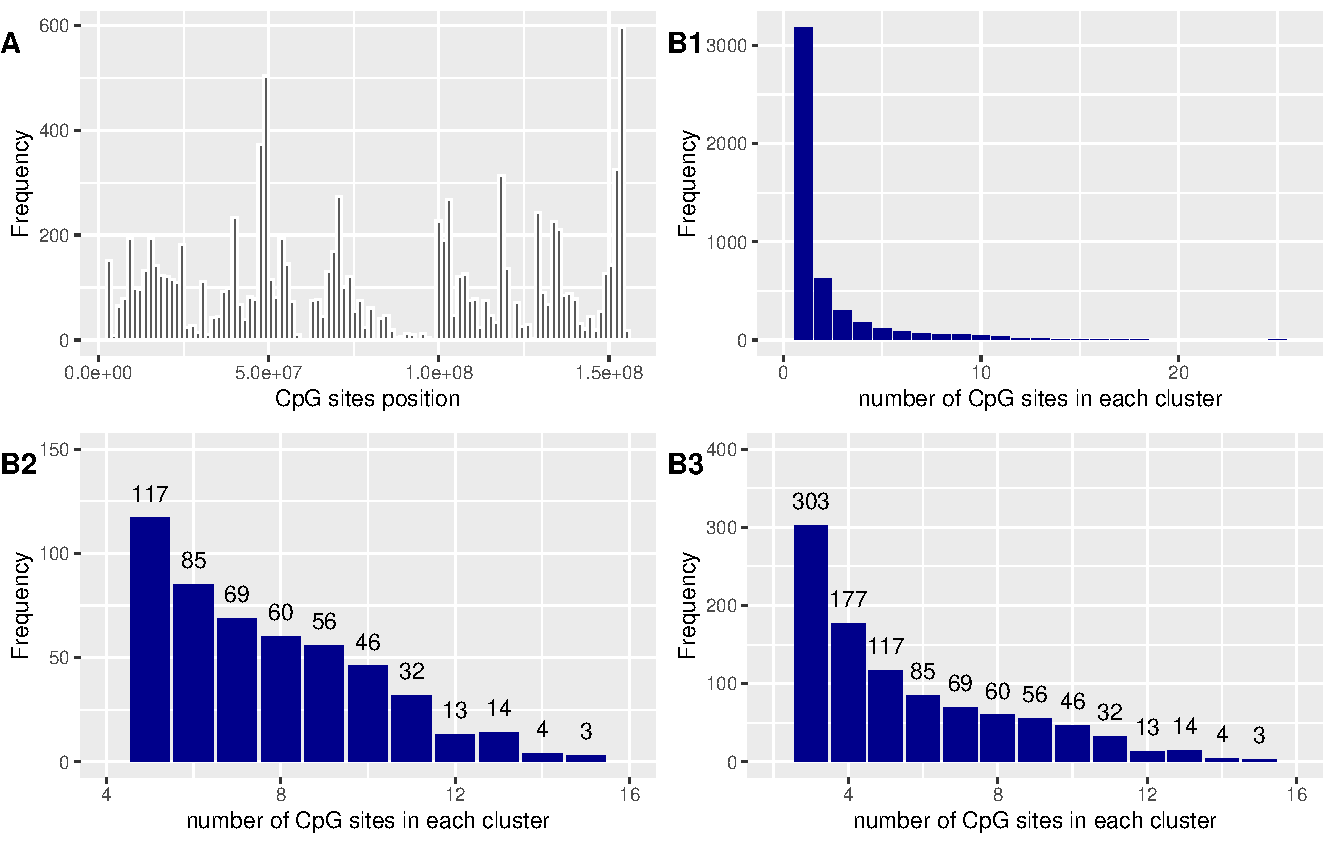
\includegraphics[scale = 0.7, trim={100 0 100 20}]{figure_cluster_lengths.pdf}
    \caption[summary statistic of cluster lengths and genetic position ]
    { \label{figure:genenetic info}
        the distribution of genetic location of sites in $S$ and distribution of cluster length of $\mathcal{C}_{500}$
        \par \small
    (A) The genetic location of CpG sites in $S$, the sites location $s_l$ is on the $x$ axis
    (B1) The distribution of cluster lengths of $\mathcal{C}_{500}$ \\
    (B2) The distribution of cluster lengths of $\mathcal{C}_{500}$, where only clusters with length $3$ to $15$ are considered \\
    (B3) The distributions of cluster lengths of $\mathcal{C}_{500}$, where only clusters with length $5$ to $15$ are considered
    }
\end{figure}

\section{Performance of Algorithm Under $H_0$}
\par
 To investigate the performance of the DMR identification algorithm under $H_0$, we conducted 100 trials of simulation.
For each trial generated 30 paired samples with no DMRs with Algorithm\ref{algorithm : simulation} by setting
parameter $n$ to $0$. Then we calculated the FPR by calculating the proportion of trials where at least one
candidate DMR is identified as a real DMR.

\subsection{Distribution of Samples Under $H_0$}
\par
To demonstrate the distribution of samples generated, we summarized the distribution of methylation level across the sites for in the  Figure \ref{figure: null samples}. The panel \textbf{A} is the histogram of site-level mean
methylation across across all CpG sites. Since the sample are simulated from multivariate normal distribution with
mean of $\mathbf{0}$, the histogram is of the expected shape. The panel \textbf{B} is the plots of mean methylation levels
across all CpG sites. Since all cluster are simulated with the same parameters, so we should not observe trend for methylation levels across CpG sites. The panel \textbf{C1} and \textbf{C2} are the histogram and scatter plot of the first paired sample. Since by \eqref{eqantion : statistical definiton}
$\Cov{X_1,X_2} = \Var{Z}\E{W_1}\E{W_2}$ and we would expect there is no correlation between two samples, for $\E{W_1} = \E{W_2} = 0$ in this case.
\begin{figure}
    \centering
    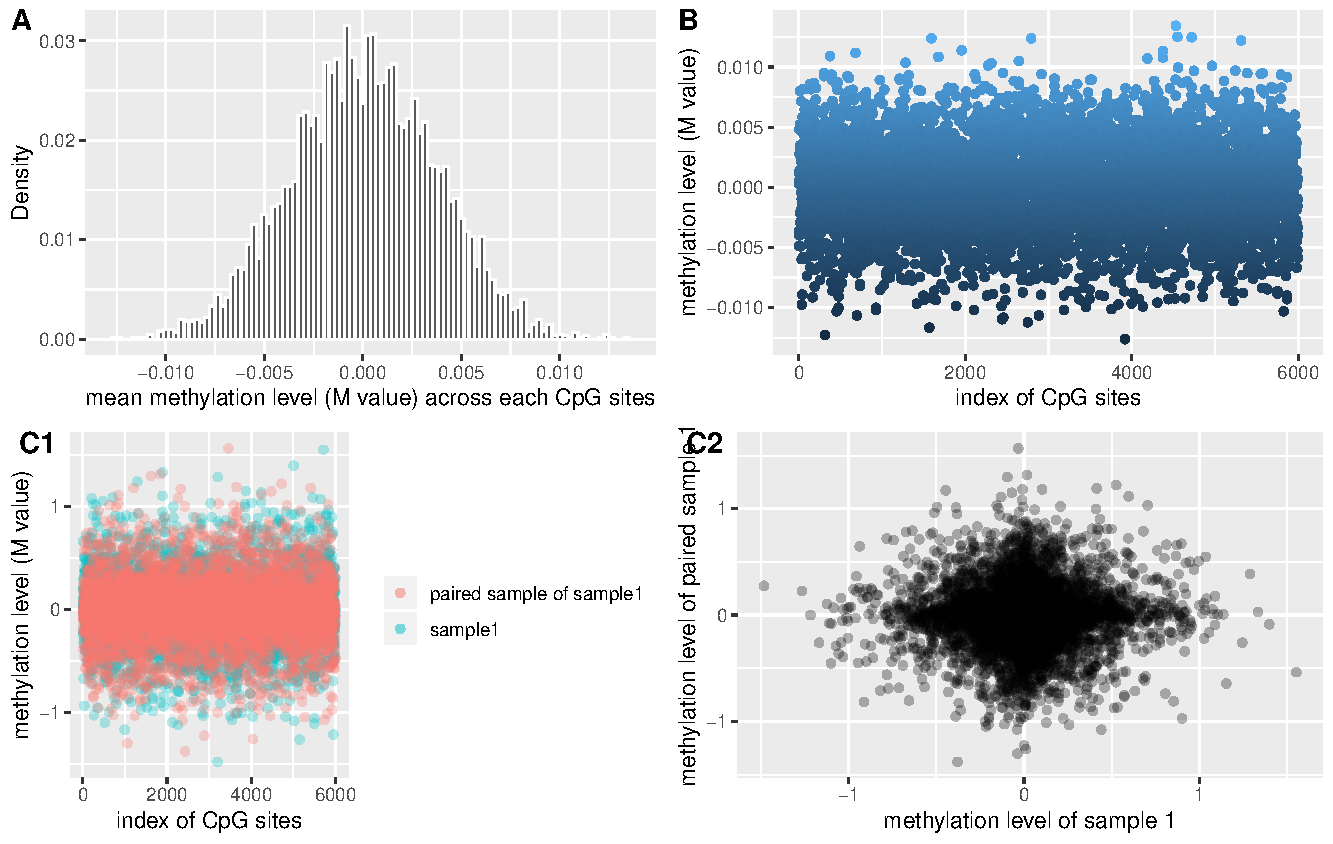
\includegraphics[scale = 0.7, trim={10 0 10 20}]{plot_null_samples.pdf}
    \caption[distribution of simulated sample under $H_0$]{
        The distribution of simulated sample under $H_0$ \label{figure: null samples}
        \par \small
        (A) The histogram of mean methylation level across all CpG sites \\
        (B) The scatter plot of mean methylation level across all CpG sites \\
        (C1) The plot of methylation level across CpG sites for the first paired sample \\
        (C2) The scatter of first paired sample against each other. The horizontal and vertical position of each
        datum represent the methylation level of certain CpG sites for the first sample and the sample
        paired with the first sample respectively.
    }
\end{figure}

\subsection{Distribution of The Significance level}
\par
We present the histogram of empirical $p$ values and FWER in the
Figure \ref{figure: null test stats}. In the 100 trials conducted, there are $5$ clusters being incorrectly identified as DMR, hence FDR is less than $0.05$. No trend is seen for the histogram of $p$ values, which is the expected result.



\begin{figure}
    \centering
    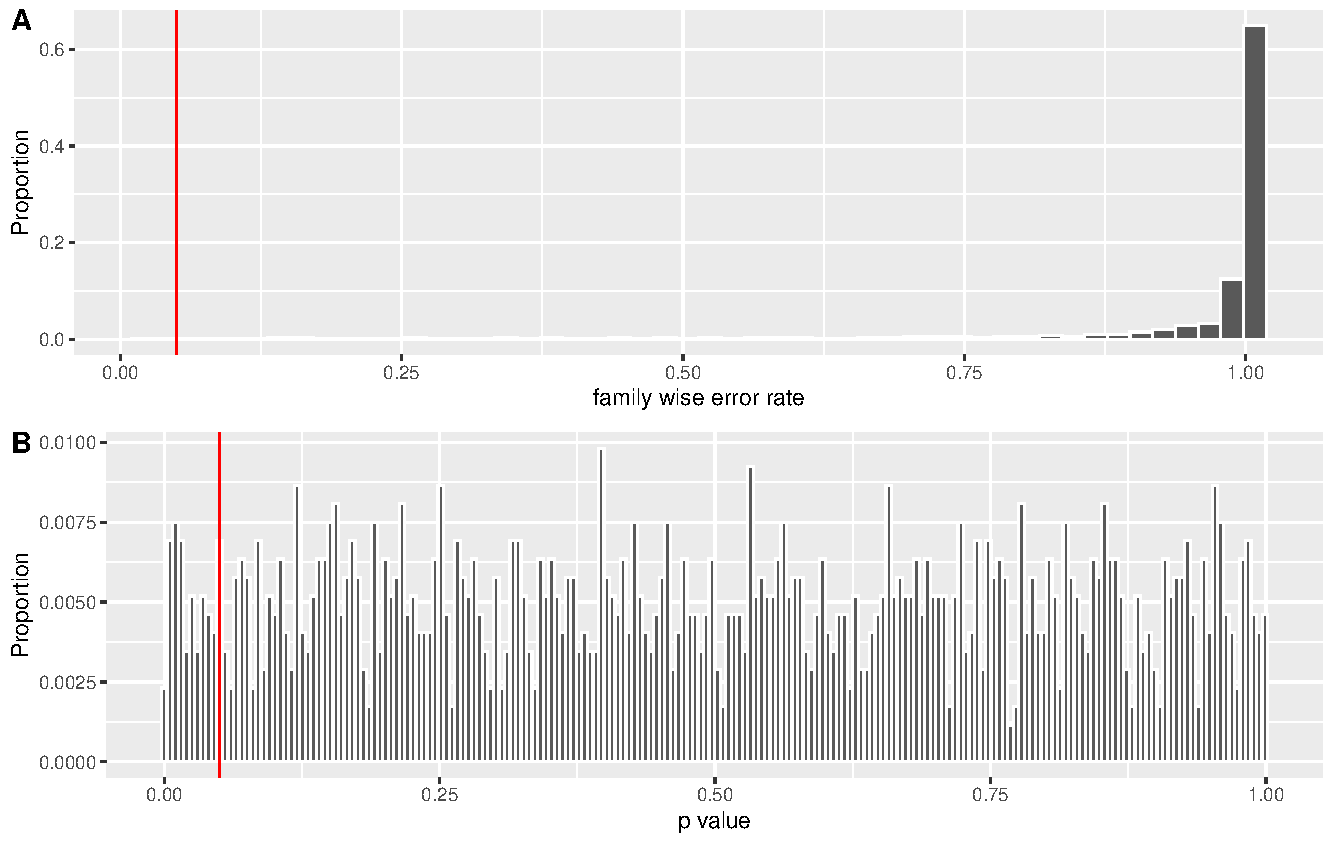
\includegraphics[scale = 0.7, trim={10 0 10 20}]{plot_eval_null.pdf}
    \caption[The distribution of significant level under $H_0$]{
        The distribution of the significant level for 100 trials, where each for each trial $30$ paired samples are generated under $H_0$ \label{figure: null test stats}
        \par \small
        (A) The histogram of empirical FWER of 100 paired trials without generating DMRs. The cutoff of FWER at $0.05$ is indicated with red vertical line.
        at $0.05$ is indicated with red vertical line.\\
        (B) The histogram of empirical $p$ values for all candidate DMRs identified. The cutoff $p$ value
        at $0.05$ is indicated with red vertical line.
    }
\end{figure}

\section{Performance of Algorithm Under $H_1$}

\subsection{Simulation With Both Mean and Variance Differences}

\par
We examined the performance of Wang's algorithm under the alternative hypothesis
with parameter $\mu_1 =1.5$ and $\delta =1.5$( \eqref{equation : parameter simulation for DMR1} and \eqref{equation : parameter simulation for DMR2}).
 We considered the cases where the length of cluster length are of $5$ to $15$ by setting subset of $\mathcal{C}_{500}$ which contains only clusters of $5$ to $15$ CpG sites as
parameter $\mathcal{C}_M$ of the Algorithm \ref{algorithm : generating candidate DMRs}; the number of DMR simulated $n$ is set to $10$ for all trials. We have conducted 10 trials, where for each trial a fixed $\mathcal{D}$ is selected and 
Algorithm \ref{algorithm : simulation} is run for $10$ times to generate 10 set of paired samples, where for each set, $30$ paired samples are generated.
Then we appled the Algorithm \ref{algorithm : Assess significance} to all samples generated and calculated TPR and TPR for each run. We then take the average of TPR, FDR and summarize them in the Table \ref{table algorithm performance}. The FDR is calculated by the proportion of the trials with no non DMR clusters being identified as DMR.
We present the histogram and scatter plot of the site-wise mean value of methylation of the first trial and the scatter plot for the first paired sample of the first trial
in the Figure \ref{figure:simulation a, 5-15}. A similar procedure is done with cluster with length $3$ to $15$.
\subsection{Simulation With Variance Differences Only}
\par
 To investigate the performance of the algorithm under the scenario where the methylation
 level of sites in DMRs for tumor and the normal tissues are of the same level but with different variably, 
 we conducted several trials by fixing $\mu_1 =0$ and vary the choice of $\delta$. Similar to the scenario with both mean and variance differences, we summary the sample generated for the first trial and the first paired in the Figure \ref{figure:simulation var only, 3-15}, \ref{figure:simulation var only, 5-15}, \ref{figure:simulation var delta5, 3-15},\ref{figure:simulation var delta5, 5-15} as an illustration of sample generated. The summary statistic of the algorithm performance indicator is given in the
 Table \ref{table algorithm performance}.

\section{Discussions and Conclusions}
\par
For our simulation, the algorithm proposed by Wang Ya et al.\cite{wang2017accounting} controls the FDR under the global $H_0$, and therefore it at least
controlled the FWER in the weak sense \cite{benjamini1995controlling}. The performance of the algorithm under the assumption $\mu_1 =1.5$ and $\delta =1.5$
agree with the result obtained by Xiao Zhang et al. \cite{zhang2018data} in their simulation. However, we found that the algorithm is  sensitive to
the distribution of the cluster length in $\mathcal{C}_M$.
\par
One reason makes their algorithm sensitive to the distribution of cluster length is the smoothing technique used in Algorithm \ref{algorithm : generating candidate DMRs}. Applying running median seems reasonable\cite{wu2015detection,hansen2012bsmooth}, but
smoothing the methylation level of sites within each cluster $C \in \mathcal{C}_M$ rather than to all the CpG sites seems a unusual choice. The default
smoothing window size is set to $5$ in the sample code given by Wang Ya et.al, but they does not exclude clusters
with length $3$ to $4$ when testing type-1 error \cite{wang2017accounting}. Since the running median method can not
be applied to a sequence of number less than the smoothing window, any clusters with length $3$ to $4$ will be set
to \verb|NA| and therefore will be impossible to be identified as DMR. The algorithm has a better performance by excluding cluster with length less than $5$ as shown in in the Table \ref{table algorithm performance}. This is not a surprising result, since clusters with length less than $5$ can not be be identified as DMR, and therefore by excluding clusters with length less than $5$ from $\mathcal{C}_M$, every simulated DMR is possible to be identified.
In Wang Ya et.al 's generalization to the case control study, they generated 10 DMRs of size 10 for their simulation study. Since the distribution of cluster length is highly right skewed as shown in the Figure \ref{figure:genenetic info}, simulation considered DMR with size $10$ only may not be a accurate reflection of the reality.
\par
In our simulation, Wang 's algorithm does not work under the scenario where methylation level of DMR sites of tumor tissue and paired normal tissue is only different in its variability($\mu_1 = 0$), as shown in the Table \ref{table algorithm performance}. In fact, the FPR is so high that the algorithm is practically not usable and the performance of the algorithm did not improve with the increased parameter $\delta$, as shown in the Table \ref{table algorithm performance} and
 Figure \ref{figure:simulation var only, 3-15}, \ref{figure:simulation var only, 5-15} \ref{figure:simulation var delta5, 5-15}.
 We have not found a satisfying explanation for the poor performance and a possible reason is, there exist a confounder between the variability of methylation level and the algorithm performance which failed to be controlled during the simulation.
 \par
Although Wang's algorithm may have a competing performance on the real methylation data, it's performance it's questionable in our simulation study. In our simulated sample, the DMRs are almost obvious for the naked eyes of human as shown in Figure \ref{figure:simulation var delta5, 5-15} and Figure \ref{figure:simulation a, 5-15}, so it's surprising that the algorithm does not have a better performance. It shall be noted that, we set permutation number $B$ to be $250$ as oppose to $1000$ as done by Wang Ya et al.\cite{wang2017accounting}, which may be an important factor causing the difference of performance in our simulation and the result Wang Ya et al. obtained.
\par
The major limitation of of our study is the small sample size. The decreased permutation number for each run and the small total trial numbers weakened the strength of the conclusion we draw from the simulations. Furthermore, a better approach to evaluate the algorithm performance with different parameters 
is to produce a ROC graph, but this requires far more data than we currently able to generate given the time constrain.
\par
Although the algorithm proposed by Wang Ya et al.does not have a good performance in our simulation studies, they did give an flexible statistical model for simulating methylation measure for each predefined cluster (\ref{eqantion : statistical definiton}) \cite{wang2017accounting}. Although the simulated samples with this model is not invariant to the choice of cluster collection $\mathcal{C}_M$, it did provide a method to characterize the spatially distributed CpG island using the concepts of clusters. Therefore, for the future work on DNA methylation, the model proposed by Wang Ya et al.can be used for modeling DMRs.

\begin{table}[ht]
    \centering{\caption{Algorithm performance summary \label{table algorithm performance}}}
     \centering
     \begin{tabular}{ c c c c c c c c}
          \toprule
          \multicolumn{3}{c}{simulation parameter} & & \multicolumn{3}{c}{performance indicator} \\
          \cline{1-3} \cline{5-7}
          $\mu_1$ & $\delta$ & cluster length range &  & TPR & PPV & FDR \\
          \midrule
          1.5 & 1.5 & $[3,15]$ & & $0.69$ & $0.922$ & $0.19$ \\
          1.5 & 1.5 & $[5,15]$ & & $0.99$ & $0.951$ & $0.01$ \\
          0   & 1.5 & $[3,15]$ & & $0.00$ & $0.00$ & $0.45$  \\
          0   & 1.5 & $[5,15]$ & & $0.03$ & $0.020$ & $0.54$ \\
          0  & 5   & $[3,15]$ & & $0.00$ & $0.00$ & $0.40$  \\
          0  & 5   & $[5,15]$ & & $0.00$ & $0.00$ & $0.47$  \\
        \bottomrule
     \end{tabular}
\end{table}




\begin{figure}
    \centering
    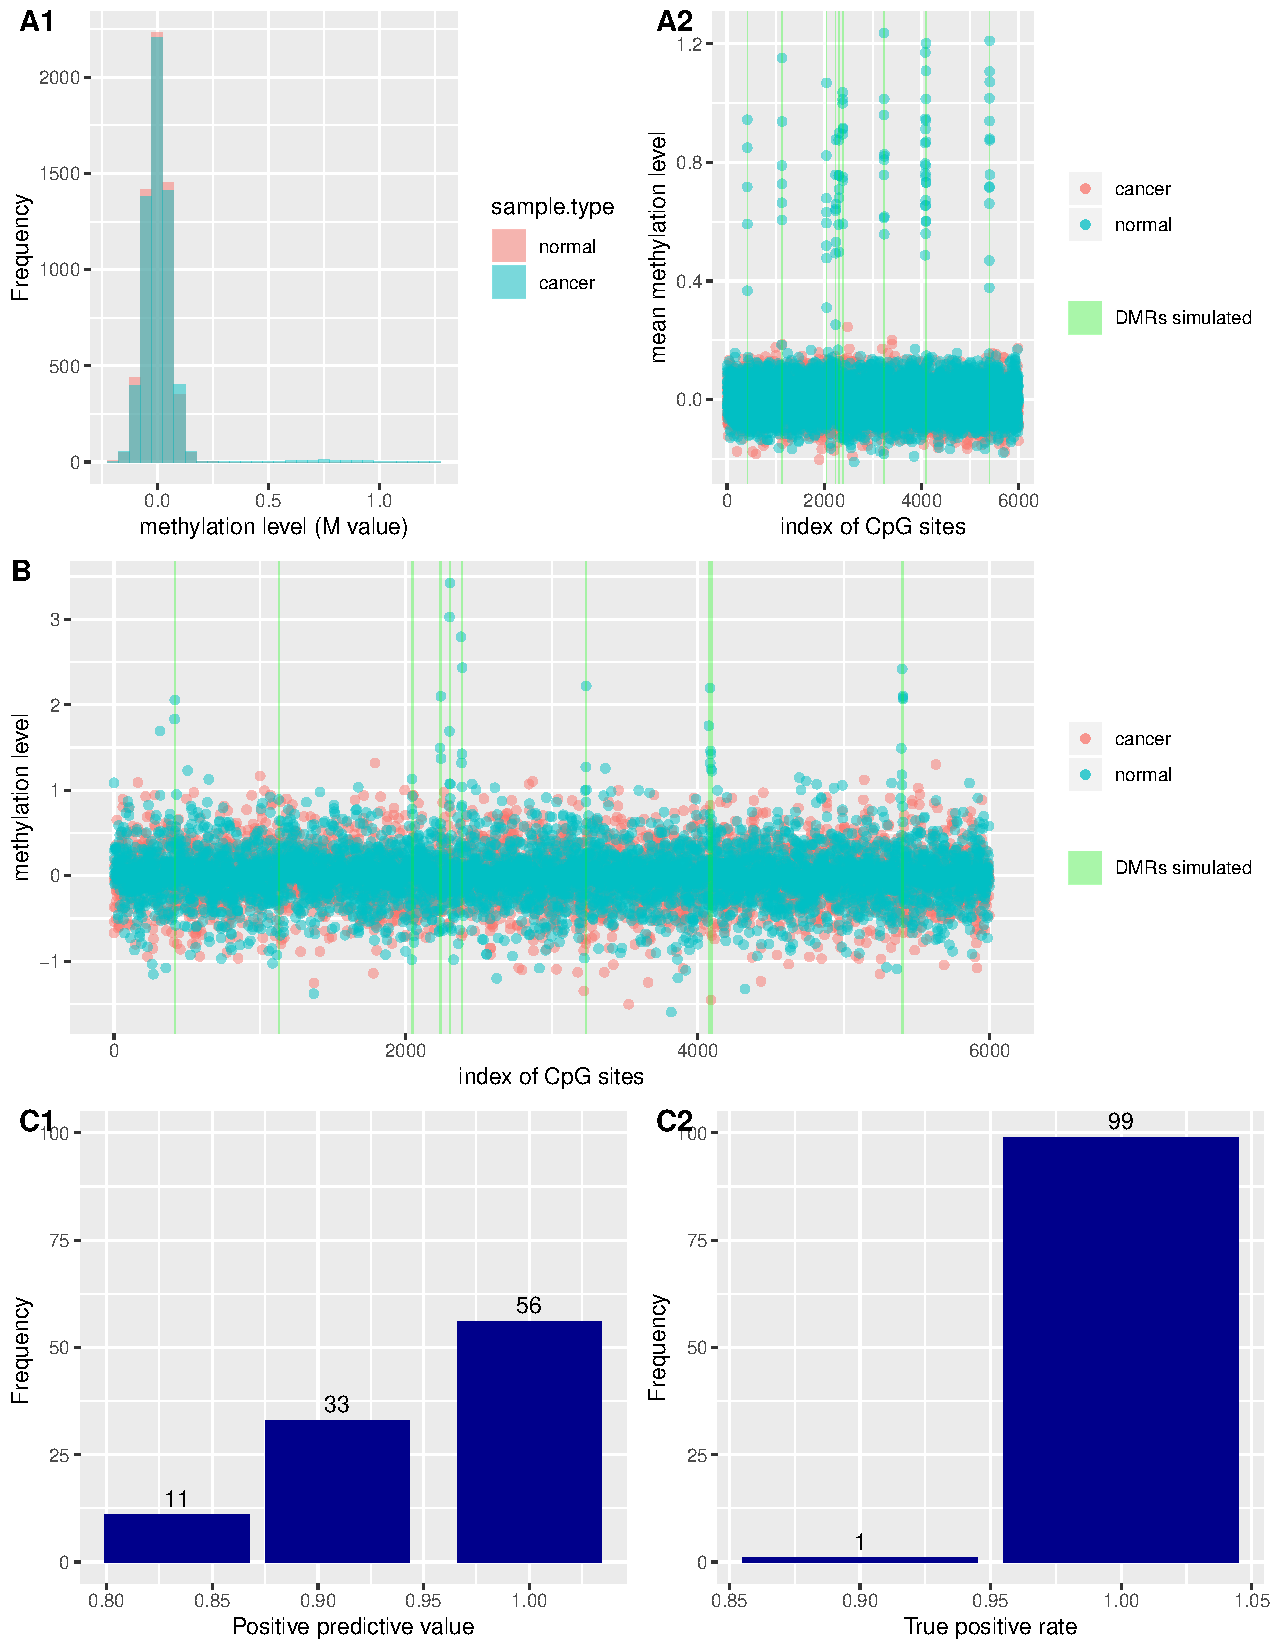
\includegraphics[scale = 0.7, trim={10 0 10 20}]{plot_sim_a.pdf}
    \caption[Result of simulation $\mu_1 = 1$ and $\delta = 1.5$]{
        Simulation result for case $\mu_1 = 1$ and $\delta = 1.5$ with cluster lengths vary from $5$ to $15$ \label{figure:simulation a, 5-15}
        \par \small
        (A1) The histogram of mean DMR level for CpG sites for normal samples and tumor tissues for the first trial.\\
        (A2) The scatter plot of mean methylation generated for the first trial. The region of DMRs selected is colored in green. \\
        (B) The scatter  plot of methylation level for the first paired example \\
        (C1 and C2) The histogram for the PPV and TPR of this 100 trials.
    }
\end{figure}

\begin{figure}
    \centering
    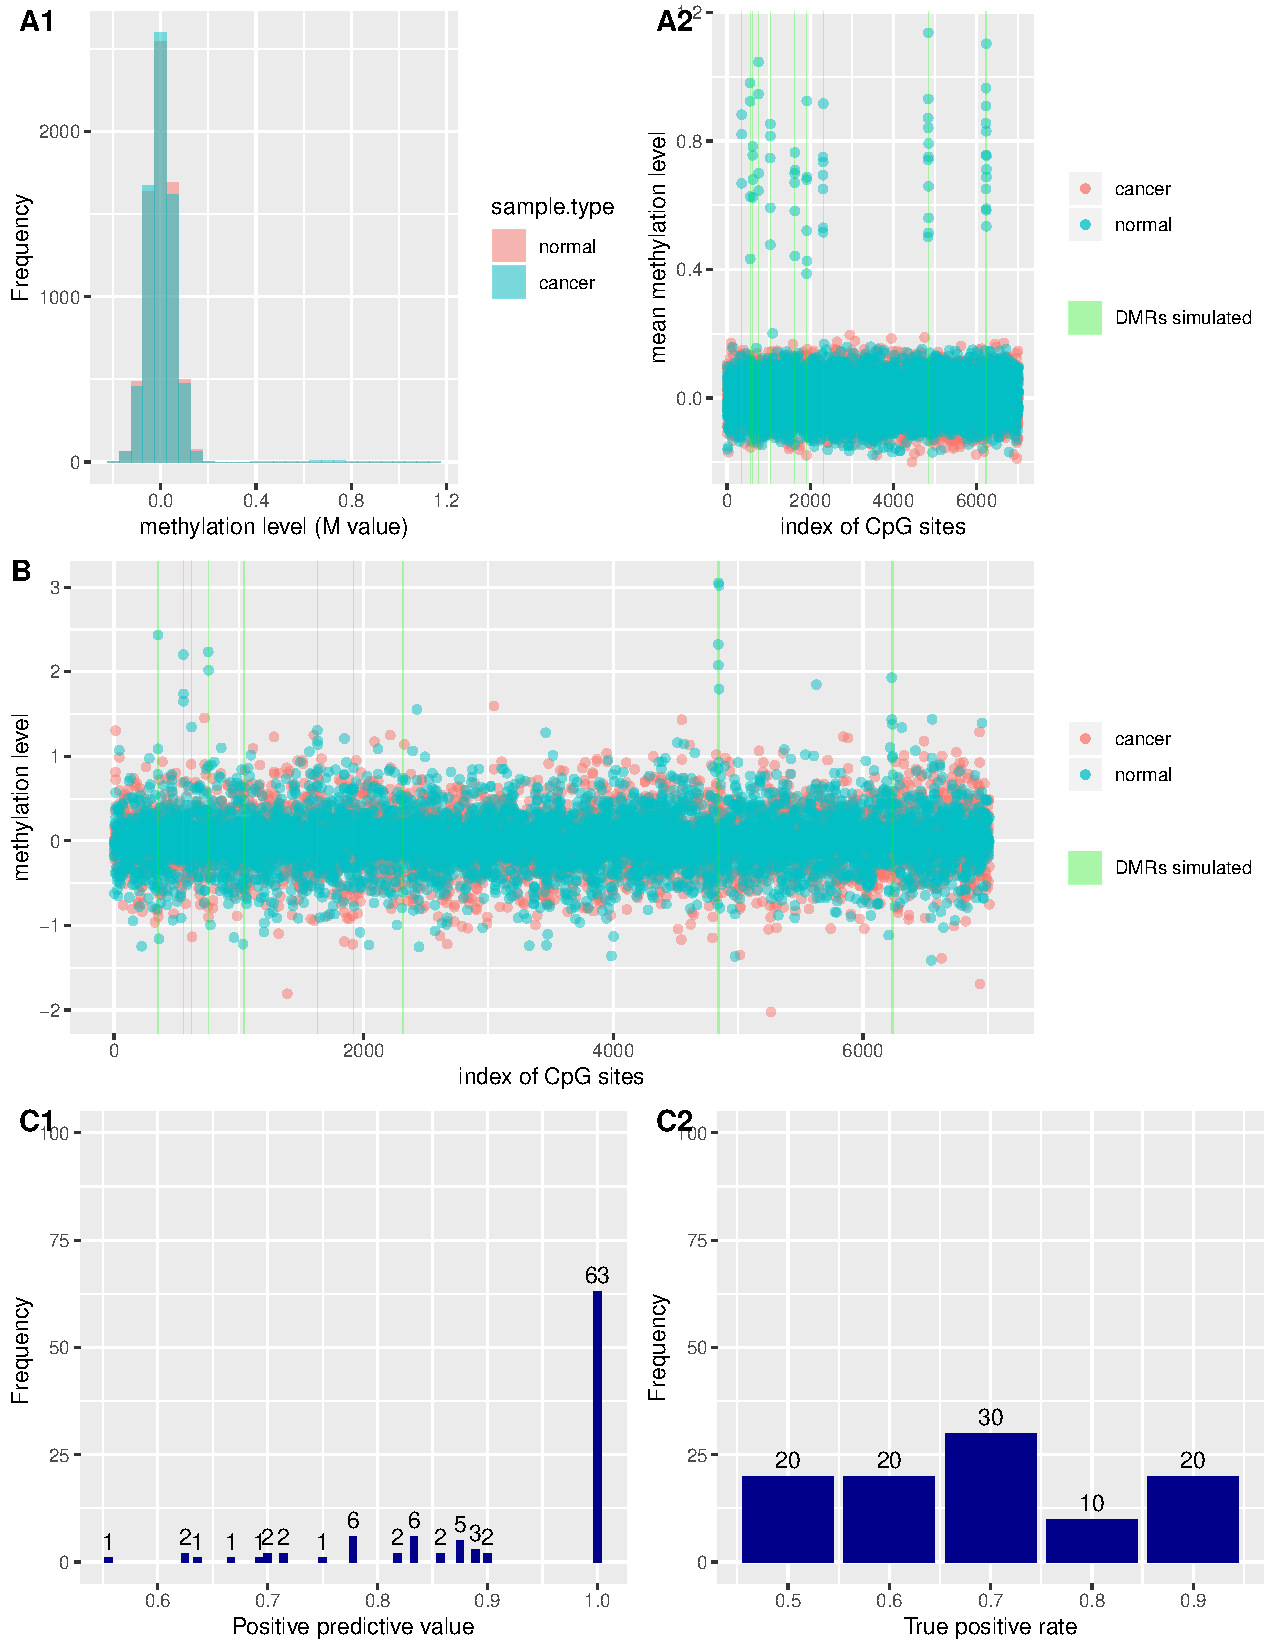
\includegraphics[scale = 0.7, trim={10 0 10 20}]{plot_sim_a_3.pdf}
    \caption[Result of simulation $\mu_1 = 1$ and $\delta = 1.5$]{
        Simulation result for case $\mu_1 = 1$ and $\delta = 1.5$ with cluster lengths vary from $3$ to $15$ \label{figure:simulation a, 3-15}
        \par \small
        (A1) The histogram of mean DMR level for CpG sites for normal samples and tumor tissues for the first trial.\\
        (A2) The scatter plot of mean methylation generated for the first trial. The region of DMRs selected is colored in green. \\
        (B) The scatter  plot of methylation level for the first paired example \\
        (C1 and C2) The histogram for the PPV and TPR of this 100 trials.
    }
\end{figure}


\begin{figure}
    \centering
    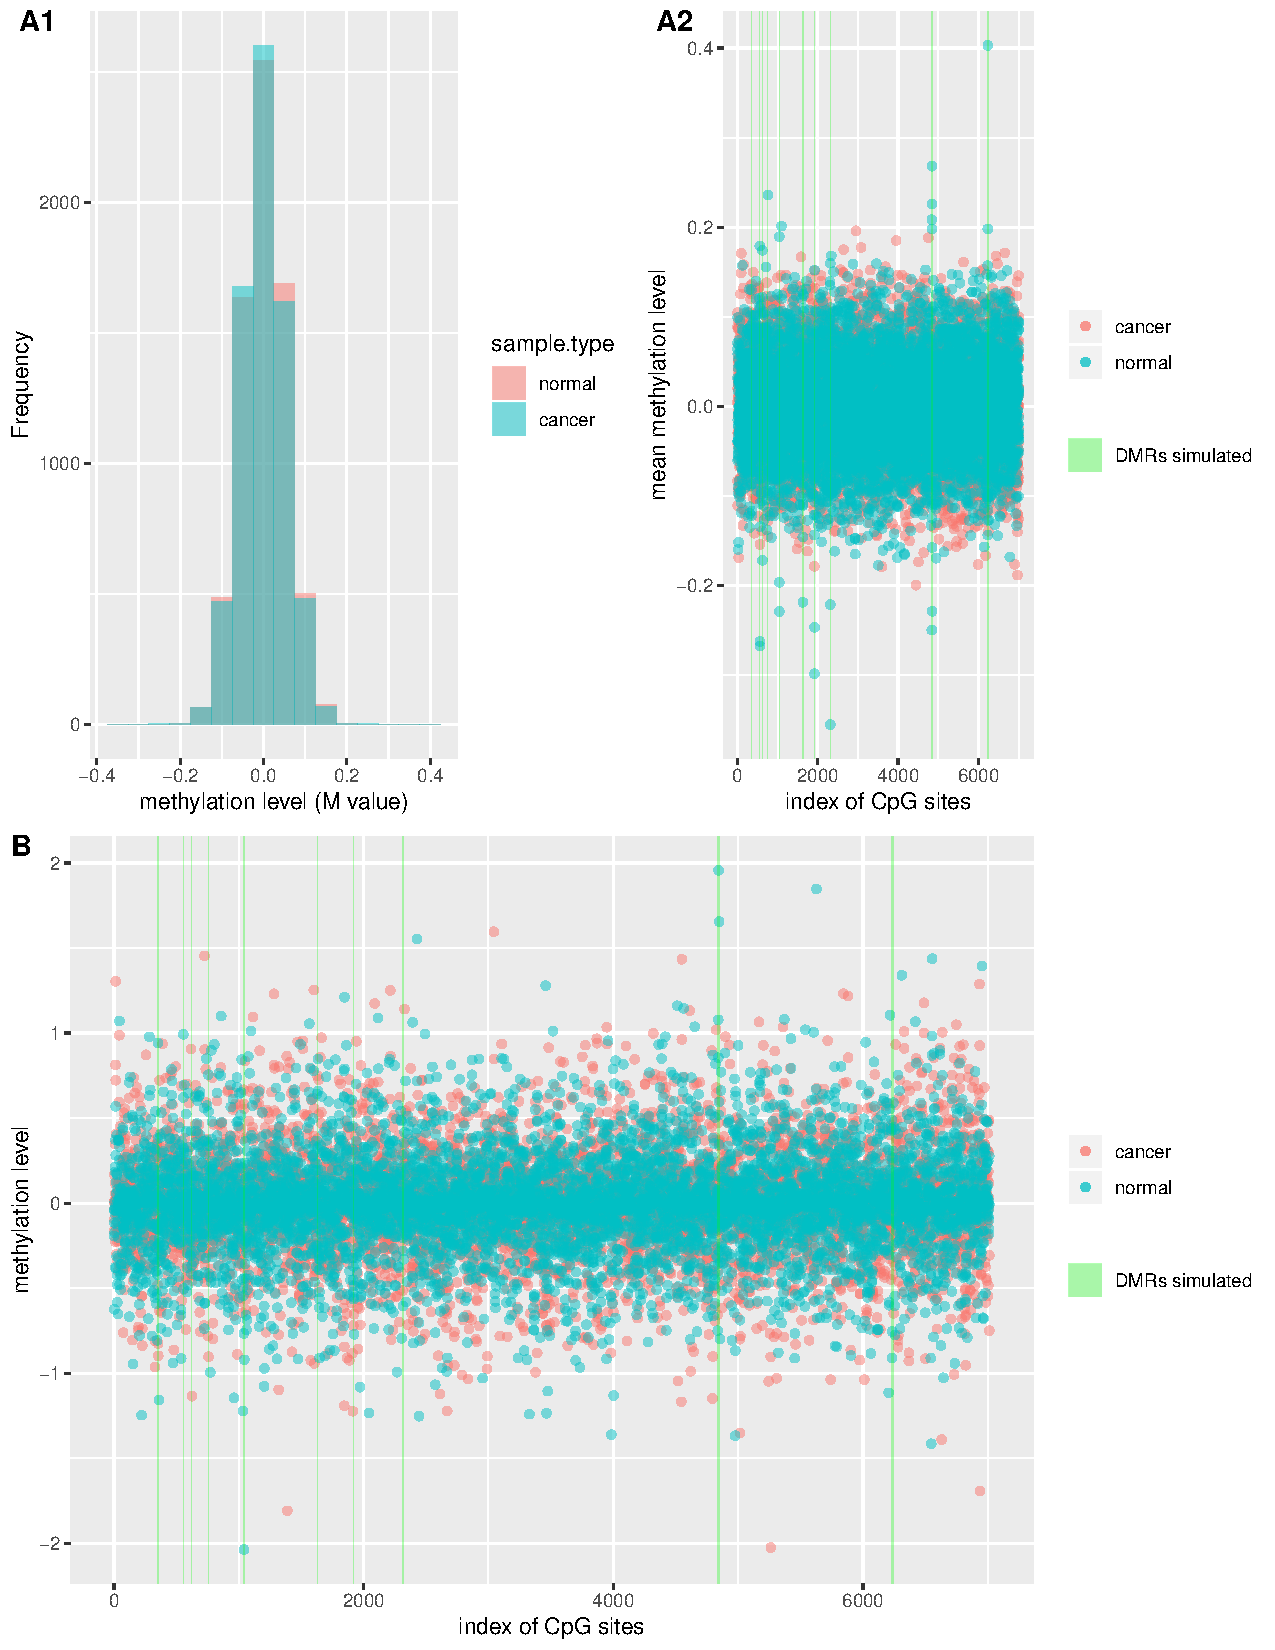
\includegraphics[scale = 0.7, trim={10 0 10 20}]{plot_var_3.pdf}
    \caption[Result of simulation $\mu_1 = 0$ and $\delta = 1.5$]{
        Simulation result for case $\mu_1 = 0$ and $\delta = 1.5$ with cluster lengths vary from $3$ to $15$ \label{figure:simulation var only, 3-15}
        \par \small
      (A1) The histogram of mean DMR level for CpG sites for normal samples and tumor tissues for the first trial.\\
        (A2) The scatter plot of mean methylation generated for the first trial. The region of DMRs selected is colored in green. \\
        (B) The scatter  plot of methylation level for the first paired example \\
    }
\end{figure}

\begin{figure}
    \centering
    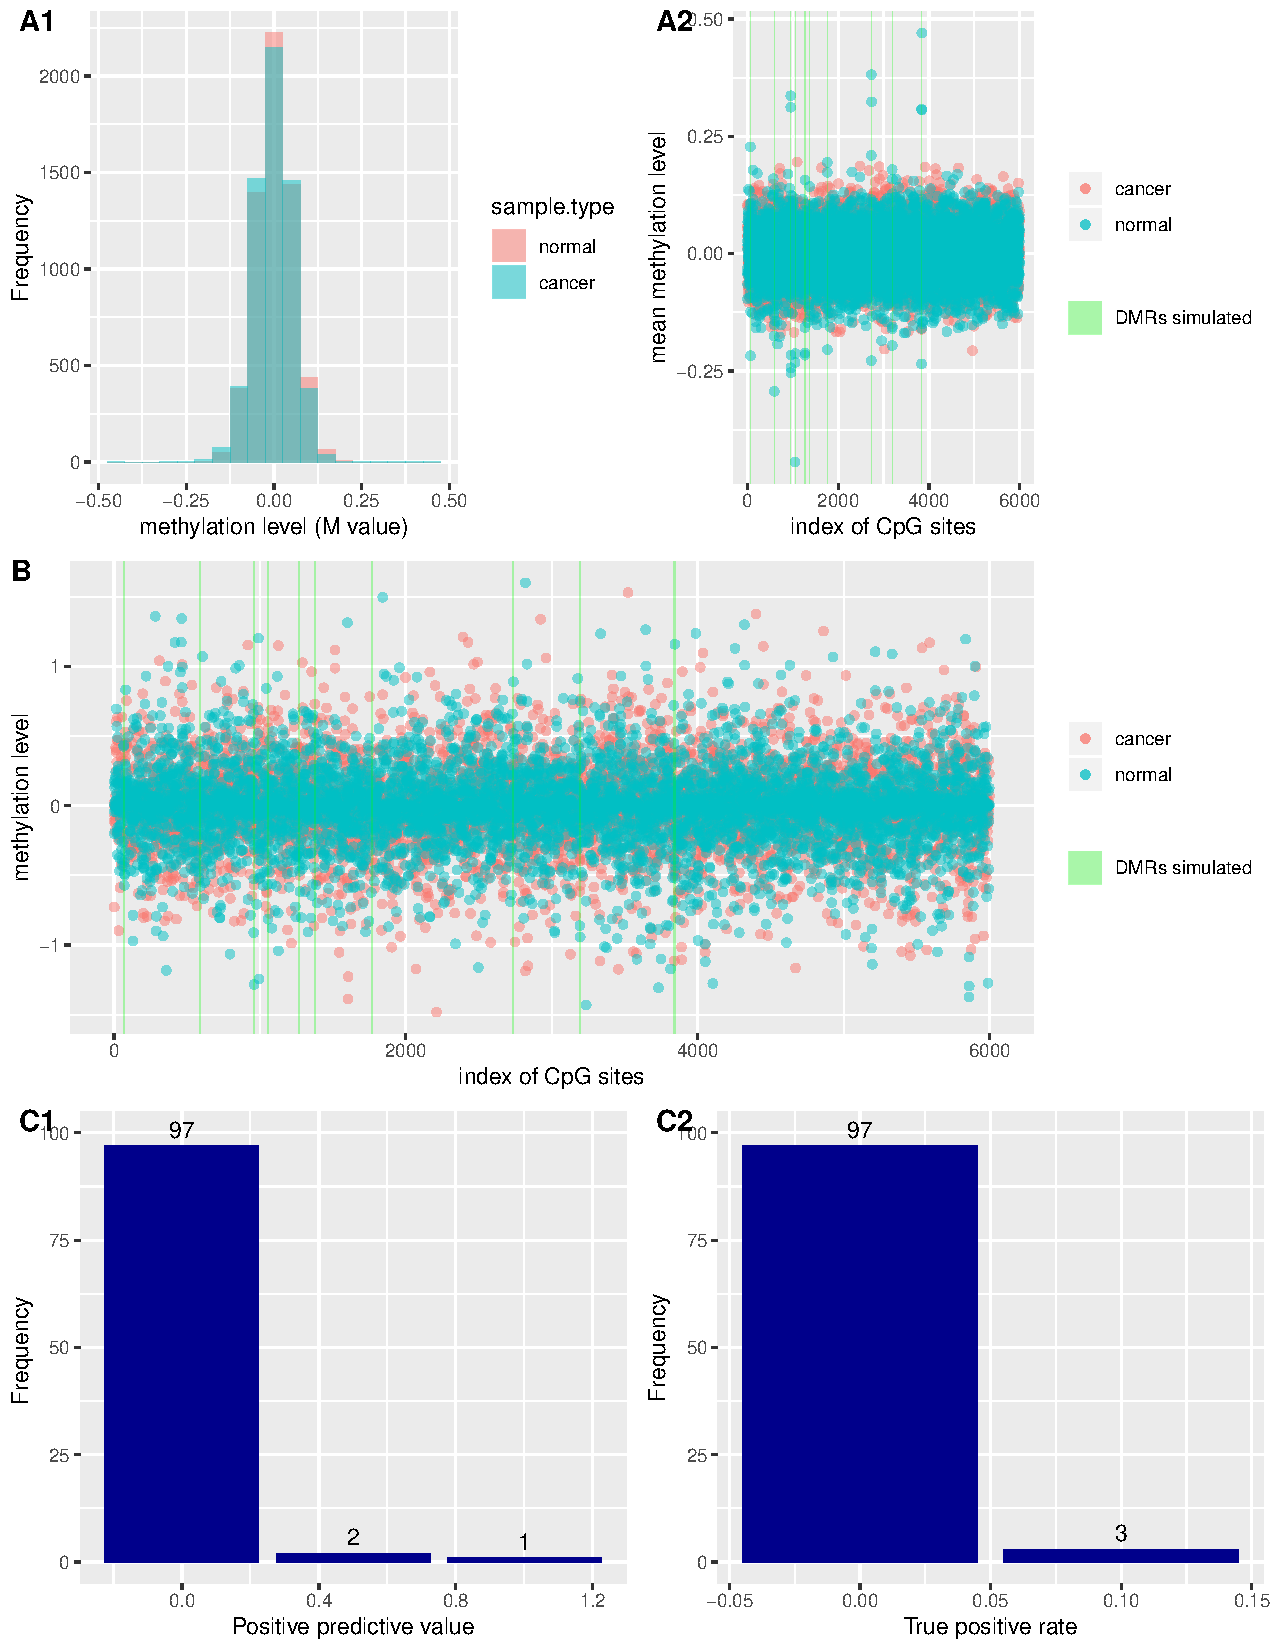
\includegraphics[scale = 0.7, trim={10 0 10 20}]{plot_var_5.pdf}
    \caption[Result of simulation $\mu_1 = 0$ and $\delta = 1.5$]{
        Simulation result for case $\mu_1 = 0$ and $\delta = 1.5$ with cluster lengths vary from $5$ to $15$ \label{figure:simulation var only, 5-15}
        \par \small
      (A1) The histogram of mean DMR level for CpG sites for normal samples and tumor tissues for the first trial.\\
        (A2) The scatter plot of mean methylation generated for the first trial. The region of DMRs selected is colored in green. \\
        (B) The scatter  plot of methylation level for the first paired example \\
    }
\end{figure}

\begin{figure}
    \centering
    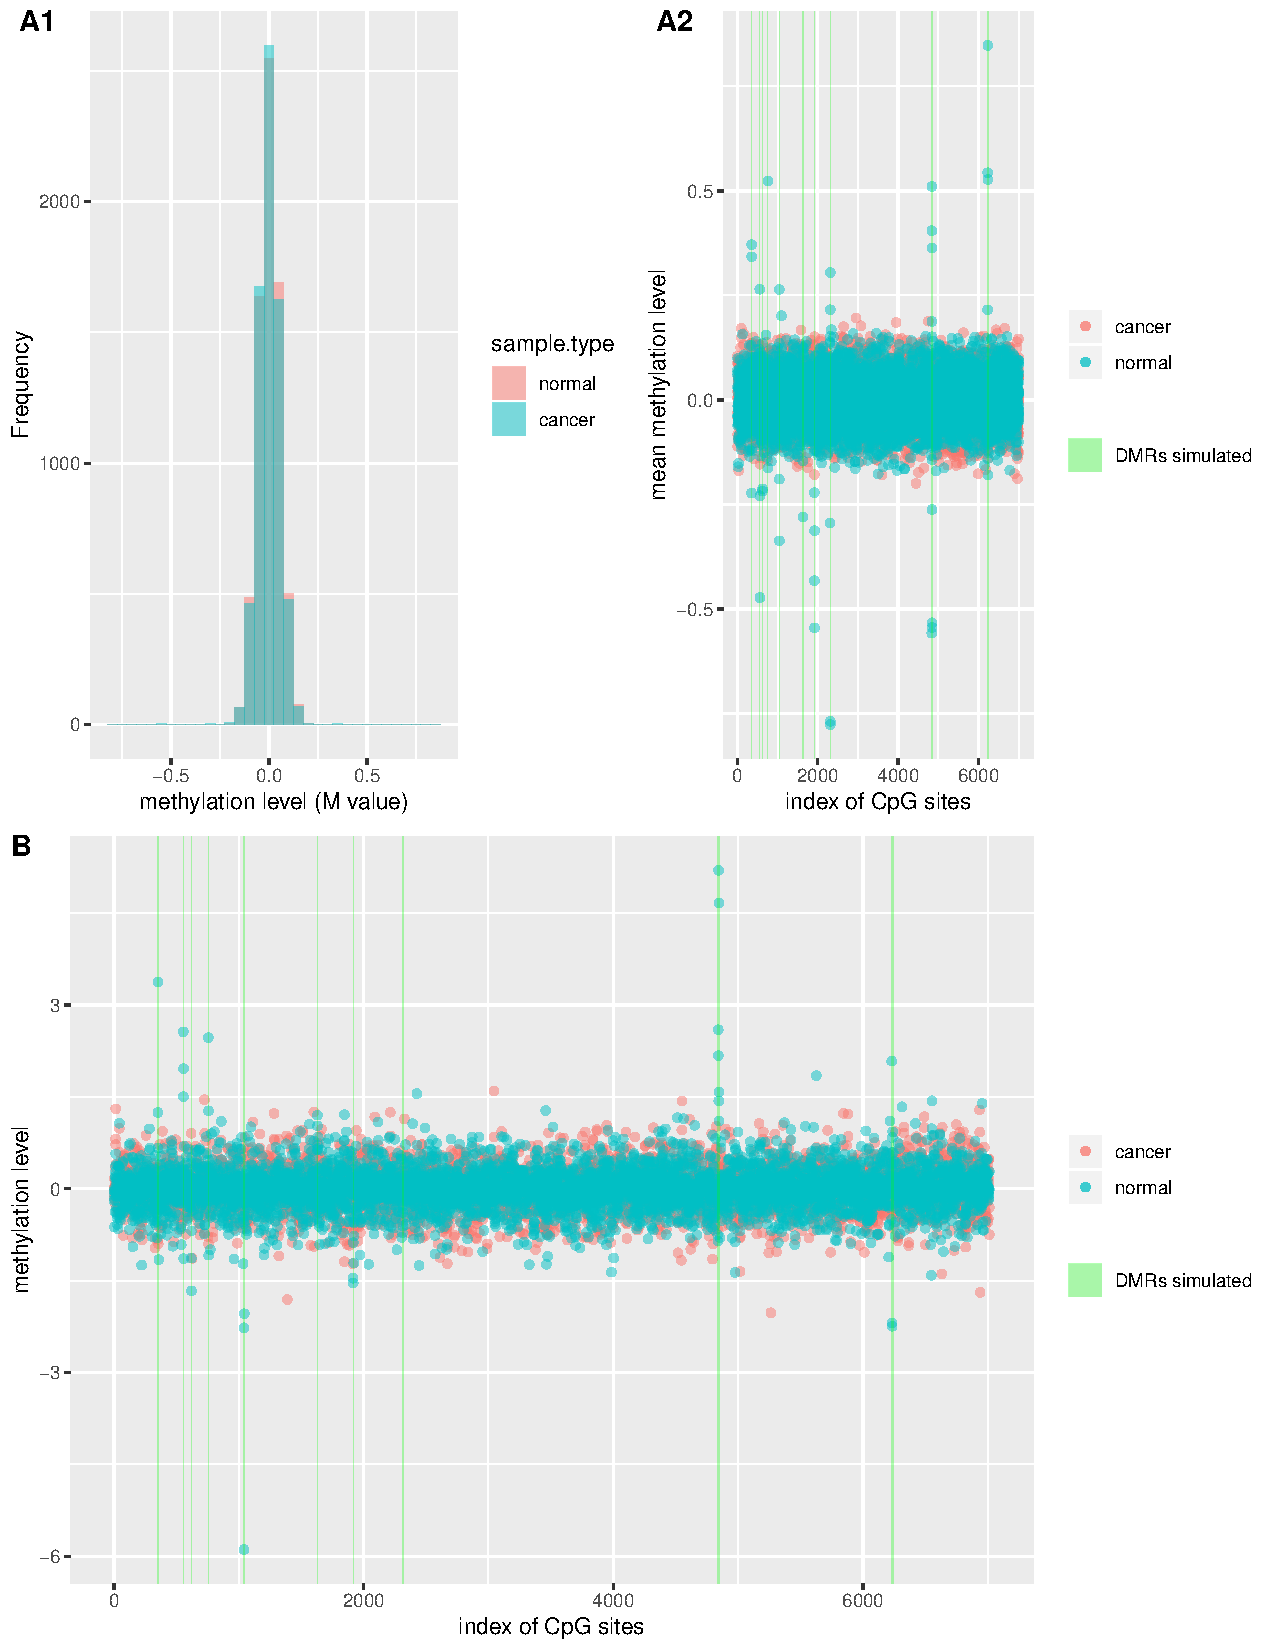
\includegraphics[scale = 0.7, trim={10 0 10 20}]{plot_var_extreme_3.pdf}
    \caption[Result of simulation $\mu_1 = 0$ and $\delta = 5$]{
        Simulation result for case $\mu_1 = 0$ and $\delta = 5$ with cluster lengths vary from $3$ to $15$ \label{figure:simulation var delta5, 3-15}
        \par \small
      (A1) The histogram of mean DMR level for CpG sites for normal samples and tumor tissues for the first trial.\\
        (A2) The scatter plot of mean methylation generated for the first trial. The region of DMRs selected is colored in green. \\
        (B) The scatter  plot of methylation level for the first paired example \\    }
\end{figure}


\begin{figure}
    \centering
    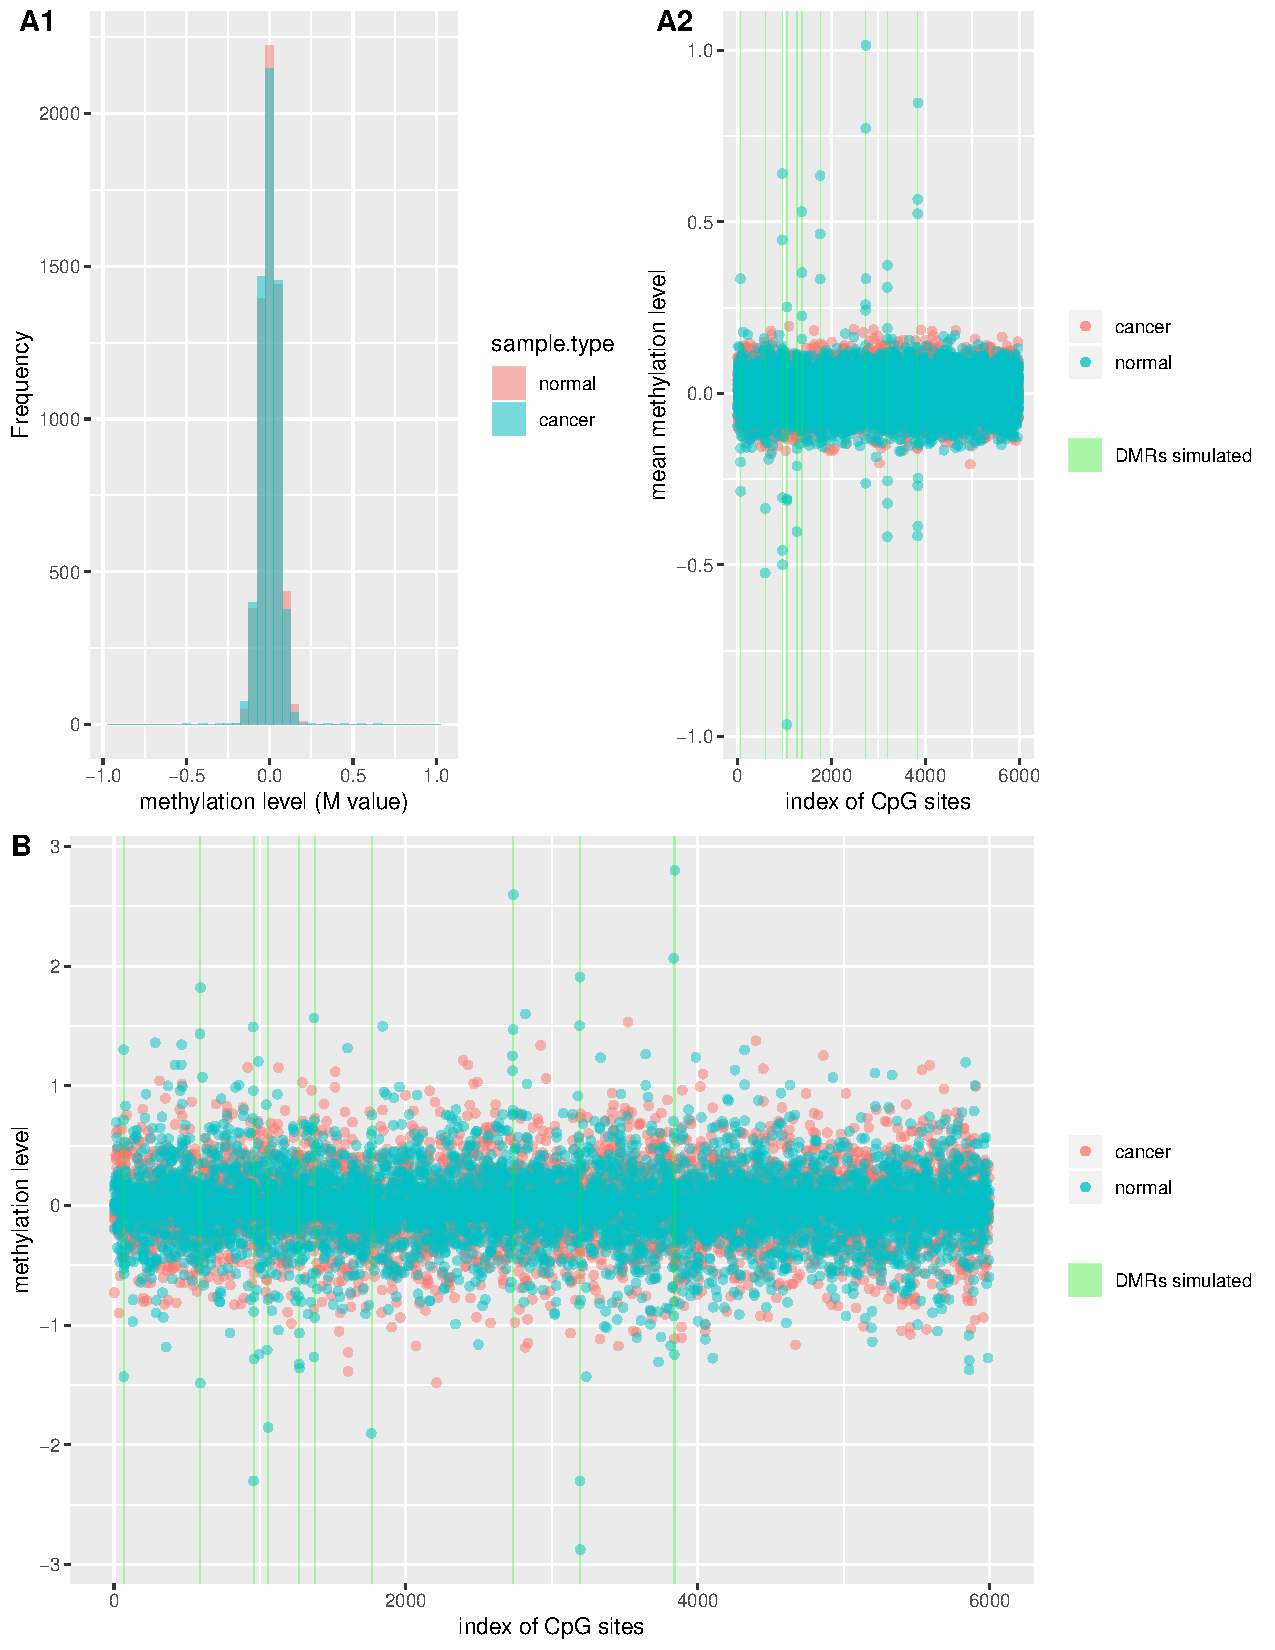
\includegraphics[scale = 0.7, trim={10 0 10 20}]{plot_var_extreme_5.pdf}
    \caption[Result of simulation $\mu_1 = 0$ and $\delta = 5$]{
        Simulation result for case $\mu_1 = 0$ and $\delta = 5$ with cluster lengths vary from $5$ to $15$ \label{figure:simulation var delta5, 5-15}
        \par \small
      (A1) The histogram of mean DMR level for CpG sites for normal samples and tumor tissues for the first trial.\\
        (A2) The scatter plot of mean methylation generated for the first trial. The region of DMRs selected is colored in green. \\
        (B) The scatter  plot of methylation level for the first paired example \\
    }
\end{figure}

\bibliographystyle{unsrt}
\bibliography{final_reportRef}
\end{document}